% -------------------------------------------------------------------------
%	PACKAGES AND OTHER DOCUMENT CONFIGURATIONS
% -------------------------------------------------------------------------

\documentclass[11pt,letter]{article}

\usepackage{fancyhdr} % Required for custom headers
\usepackage[]{geometry}
\usepackage{lastpage} % Required to determine the last page for the footer
\usepackage{extramarks} % Required for headers and footers
\usepackage[usenames,dvipsnames]{color} % Required for custom colors
\usepackage{graphicx} % Required to insert images
\usepackage{listings} % Required for insertion of code
\usepackage[round]{natbib}
% \usepackage[scaled]{helvet}
%\usepackage{couriernew} % Required for the courier font
\usepackage{booktabs}
\usepackage{amsmath}
\usepackage{url}
\usepackage{xcolor}

\usepackage[font=itshape]{quoting}

% \usepackage{mathpazo}
% \usepackage{times}
\usepackage{txfonts}
% \usepackage{mathptmx}
% \usepackage[scaled=0.9]{DejaVuSansMono}
% \usepackage[]{inconsolata}

\usepackage{enumerate} % Required for enumerating with letters

\usepackage{setspace}

% -------------------------------------------------------------------------
% Homework name, etc.

\newcommand{\sw}[1]{\textcolor{blue}{#1}}

\newcommand{\W}{\mathbf{W}}
\newcommand{\Y}{\mathbf{Y}}
\newcommand{\X}{\mathbf{X}}
\newcommand{\Z}{\mathbf{Z}}

\newcommand{\mis}{\text{mis}}
\newcommand{\obs}{\text{obs}}

\newcommand{\dif}{\text{dif}}
\newcommand{\rank}{\text{rank}}
\newcommand{\gain}{\text{gain}}

\newcommand{\OT}{O\textsubscript{3}}

\newcommand{\hmwkTitle}{Homework~2} % Assignment title
\newcommand{\hmwkDueDate}{March 24, 2020} % Due date


\newcommand{\hmwkClass}{SDS 384: Causal Inference Methodology} % Course/class
\newcommand{\hmwkClassTime}{} % Class/lecture time
\newcommand{\hmwkClassInstructor}{Professor Zigler} % Teacher/lecturer
\newcommand{\hmwkAuthorName}{Spencer Woody} % Your name

\newcommand\ind{\protect\mathpalette{\protect\independenT}{\perp}}
\def\independenT#1#2{\mathrel{\rlap{$#1#2$}\mkern2mu{#1#2}}}


% -------------------------------------------------------------------------
% Source in format




% Specify sans body text, math serif text
\documentclass[sans, mathserif, professionalfont, 11pt]{beamer}

% \documentclass[sans]{beamer}

% \documentclass{beamer}

% Specify fonts
% \usepackage[default]{roboto}
% \usepackage[scaled]{helvet} % Sans sefif body text
\usepackage{txfonts}
\usepackage[scaled]{helvet} % Sans sefif body text
% \usepackage[]{comicneue} % Sans sefif body text
% \usepackage{cmbright}
% \usepackage[default]{comicneue}
% \usepackage{mathpazo} % Palatino for math
% \usepackage{eulervm}
\usepackage[scaled=0.95]{inconsolata} % Inconsolata fixed width font
% \usepackage[]{inconsolata} % Inconsolata fixed width font

% \usepackage[]{txfonts}

\usepackage{tikz}
\usepackage{ragged2e}
\usepackage{lipsum}
\usepackage{hyperref}

\justifying

% Bibliography
\usepackage[round]{natbib}
% \bibliographystyle{apacite}
\usepackage{appendixnumberbeamer}
\bibliographystyle{plainnat}
% \AtBeginDocument{\renewcommand{\harvardand}{\&}}

\newcommand\ind{\protect\mathpalette{\protect\independenT}{\perp}}
\def\independenT#1#2{\mathrel{\rlap{$#1#2$}\mkern2mu{#1#2}}}


\newcommand{\U}{\mathbf{U}}
\newcommand{\M}{\mathbf{M}}
\newcommand{\m}{\mathbf{m}}
\newcommand{\w}{\mathbf{w}}

\newcommand{\N}{\mathcal{N}}
\newcommand{\dee}{\mathrm{d}}
\newcommand{\F}{\mathcal{F}}
\newcommand{\trans}{\intercal}
\newcommand{\y}{\mathbf{y}}
\newcommand{\f}{\mathbf{f}}
\newcommand{\I}{\mathcal{I}}
\newcommand{\gammatilde}{\tilde{\gamma}}
\newcommand{\betabar}{\bar{\beta}}
\newcommand{\Ytilde}{\tilde{Y}}
\newcommand{\LL}{\mathcal{L}}
\newcommand{\E}{\mathrm{E}}


% Use mathbb symbols from Computer Modern
% \AtBeginDocument{
%   \DeclareSymbolFont{AMSb}{U}{msb}{m}{n}
%   \DeclareSymbolFontAlphabet{\mathbb}{AMSb}}

\DeclareMathOperator{\EE}{E}

% Graphics, tables, math, etc.
\usepackage{graphicx} 
\usepackage{booktabs} 
\usepackage{amsmath}
\usepackage{bm}
\usepackage{amssymb}
\usepackage{xcolor}

% \usepackage[symbol]{footmisc}

% \renewcommand{\thefootnote}{\fnsymbol{footnote}}

\renewcommand*{\thefootnote}{\fnsymbol{footnote}}

% Formatting
\setbeamertemplate{caption}[numbered]

\setbeamertemplate{title page}
{
  \begin{minipage}[b][\paperheight]{\textwidth}
    \vfill
    \ifx\inserttitle\@empty%
    \else%
    {\raggedright\linespread{0.8}\usebeamerfont{title}\usebeamercolor[fg]{title}
      % \scshape\MakeLowercase{\inserttitle}\par}%
      \scshape
      {\inserttitle}\par}%
    \vspace*{0.5em}
    \fi%
    \ifx\insertsubtitle\@empty%
    \else%
    {\usebeamerfont{subtitle}\usebeamercolor[fg]{subtitle}\insertsubtitle\par}%
    \vspace*{0.5em}
    \hrule
    \fi%
    \vspace*{0.5em}
    \ifx\insertauthor\@empty%
    \else%
    {\usebeamerfont{author}\usebeamercolor[fg]{author}\insertauthor\par}%
    \vspace*{0.25em}
    \fi%
    % Institute
    \ifx\insertinstitut\@empty%
    \else%
    \vspace*{3mm}
    {\usebeamerfont{institute}\usebeamercolor[fg]{institute}\insertinstitute\par}%
    \fi%
        \vspace*{3mm}
        % Date
    \ifx\insertdate\@empty%
    \else%
    {\usebeamerfont{date}\usebeamercolor[fg]{date}\insertdate\par}%
    \fi%
    \vspace*{5mm}
    % \vfill
    % -------------------------------------------------------------------------
    % -------------------------------------------------------------------------
    % -------------------------------------------------------------------------
    % -------------------------------------------------------------------------
    % University logo; if none, comment out
    \if1\graphic{
      % \begin{center}
      
\includegraphics[width=0.5\textwidth]{img/department-logo.png}\\
      % 
\includegraphics[width=0.6\textwidth]{img/McCombs_School_Brand_Branded.png}
      % 
\includegraphics[width=0.6\textwidth]{img/irom-logo.png}
      % \end{center}
    }\fi
    % -------------------------------------------------------------------------
    % -------------------------------------------------------------------------
    % -------------------------------------------------------------------------
    % -------------------------------------------------------------------------
  \vfill
  \vspace*{5mm}
  \end{minipage}
}

% \AtBeginSection{\frame{\sectionpage}}

\setbeamertemplate{frametitle}
  {\begin{flushleft}\smallskip 
    \insertframetitle\par 
   \vskip1pt\end{flushleft}}
\setbeamertemplate{itemize item}{$\bullet$}
\setbeamertemplate{navigation symbols}{}
% \setbeamertemplate{footline}[text line]{%
%     \hfill
% }
 \setbeamertemplate {footline}{\quad\hfill\insertframenumber\strut\quad}
\setbeamertemplate{footline}{
  \hfill%
  \usebeamercolor[fg]{page number in head/foot}%
  \usebeamerfont{page number in head/foot}%
  % Use this line for only the current frame number
  \setbeamertemplate{page number in head/foot}[framenumber]%
  % Use this line for frame number and *total* frame number
    % \setbeamertemplate{page number in head/foot}[totalframenumber]%
  \usebeamertemplate*{page number in head/foot}\kern1.5em\vskip8pt
}


% You can customize color settings here

% % Define some colors:

% Colors from R; see following page
% http://research.stowers.org/mcm/efg/R/Color/Chart/ColorChart.pdf
\definecolor{white}{HTML}{FFFFFF}
\definecolor{aliceblue}{HTML}{F0F8FF}
\definecolor{antiquewhite}{HTML}{FAEBD7}
\definecolor{antiquewhite1}{HTML}{FFEFDB}
\definecolor{antiquewhite2}{HTML}{EEDFCC}
\definecolor{antiquewhite3}{HTML}{CDC0B0}
\definecolor{antiquewhite4}{HTML}{8B8378}
\definecolor{aquamarine}{HTML}{7FFFD4}
\definecolor{aquamarine1}{HTML}{7FFFD4}
\definecolor{aquamarine2}{HTML}{76EEC6}
\definecolor{aquamarine3}{HTML}{66CDAA}
\definecolor{aquamarine4}{HTML}{458B74}
\definecolor{azure}{HTML}{F0FFFF}
\definecolor{azure1}{HTML}{F0FFFF}
\definecolor{azure2}{HTML}{E0EEEE}
\definecolor{azure3}{HTML}{C1CDCD}
\definecolor{azure4}{HTML}{838B8B}
\definecolor{beige}{HTML}{F5F5DC}
\definecolor{bisque}{HTML}{FFE4C4}
\definecolor{bisque1}{HTML}{FFE4C4}
\definecolor{bisque2}{HTML}{EED5B7}
\definecolor{bisque3}{HTML}{CDB79E}
\definecolor{bisque4}{HTML}{8B7D6B}
\definecolor{black}{HTML}{000000}
\definecolor{blanchedalmond}{HTML}{FFEBCD}
\definecolor{blue}{HTML}{0000FF}
\definecolor{blue1}{HTML}{0000FF}
\definecolor{blue2}{HTML}{0000EE}
\definecolor{blue3}{HTML}{0000CD}
\definecolor{blue4}{HTML}{00008B}
\definecolor{blueviolet}{HTML}{8A2BE2}
\definecolor{brown}{HTML}{A52A2A}
\definecolor{brown1}{HTML}{FF4040}
\definecolor{brown2}{HTML}{EE3B3B}
\definecolor{brown3}{HTML}{CD3333}
\definecolor{brown4}{HTML}{8B2323}
\definecolor{burlywood}{HTML}{DEB887}
\definecolor{burlywood1}{HTML}{FFD39B}
\definecolor{burlywood2}{HTML}{EEC591}
\definecolor{burlywood3}{HTML}{CDAA7D}
\definecolor{burlywood4}{HTML}{8B7355}
\definecolor{cadetblue}{HTML}{5F9EA0}
\definecolor{cadetblue1}{HTML}{98F5FF}
\definecolor{cadetblue2}{HTML}{8EE5EE}
\definecolor{cadetblue3}{HTML}{7AC5CD}
\definecolor{cadetblue4}{HTML}{53868B}
\definecolor{chartreuse}{HTML}{7FFF00}
\definecolor{chartreuse1}{HTML}{7FFF00}
\definecolor{chartreuse2}{HTML}{76EE00}
\definecolor{chartreuse3}{HTML}{66CD00}
\definecolor{chartreuse4}{HTML}{458B00}
\definecolor{chocolate}{HTML}{D2691E}
\definecolor{chocolate1}{HTML}{FF7F24}
\definecolor{chocolate2}{HTML}{EE7621}
\definecolor{chocolate3}{HTML}{CD661D}
\definecolor{chocolate4}{HTML}{8B4513}
\definecolor{coral}{HTML}{FF7F50}
\definecolor{coral1}{HTML}{FF7256}
\definecolor{coral2}{HTML}{EE6A50}
\definecolor{coral3}{HTML}{CD5B45}
\definecolor{coral4}{HTML}{8B3E2F}
\definecolor{cornflowerblue}{HTML}{6495ED}
\definecolor{cornsilk}{HTML}{FFF8DC}
\definecolor{cornsilk1}{HTML}{FFF8DC}
\definecolor{cornsilk2}{HTML}{EEE8CD}
\definecolor{cornsilk3}{HTML}{CDC8B1}
\definecolor{cornsilk4}{HTML}{8B8878}
\definecolor{cyan}{HTML}{00FFFF}
\definecolor{cyan1}{HTML}{00FFFF}
\definecolor{cyan2}{HTML}{00EEEE}
\definecolor{cyan3}{HTML}{00CDCD}
\definecolor{cyan4}{HTML}{008B8B}
\definecolor{darkblue}{HTML}{00008B}
\definecolor{darkcyan}{HTML}{008B8B}
\definecolor{darkgoldenrod}{HTML}{B8860B}
\definecolor{darkgoldenrod1}{HTML}{FFB90F}
\definecolor{darkgoldenrod2}{HTML}{EEAD0E}
\definecolor{darkgoldenrod3}{HTML}{CD950C}
\definecolor{darkgoldenrod4}{HTML}{8B6508}
\definecolor{darkgray}{HTML}{A9A9A9}
\definecolor{darkgreen}{HTML}{006400}
\definecolor{darkgrey}{HTML}{A9A9A9}
\definecolor{darkkhaki}{HTML}{BDB76B}
\definecolor{darkmagenta}{HTML}{8B008B}
\definecolor{darkolivegreen}{HTML}{556B2F}
\definecolor{darkolivegreen1}{HTML}{CAFF70}
\definecolor{darkolivegreen2}{HTML}{BCEE68}
\definecolor{darkolivegreen3}{HTML}{A2CD5A}
\definecolor{darkolivegreen4}{HTML}{6E8B3D}
\definecolor{darkorange}{HTML}{FF8C00}
\definecolor{darkorange1}{HTML}{FF7F00}
\definecolor{darkorange2}{HTML}{EE7600}
\definecolor{darkorange3}{HTML}{CD6600}
\definecolor{darkorange4}{HTML}{8B4500}
\definecolor{darkorchid}{HTML}{9932CC}
\definecolor{darkorchid1}{HTML}{BF3EFF}
\definecolor{darkorchid2}{HTML}{B23AEE}
\definecolor{darkorchid3}{HTML}{9A32CD}
\definecolor{darkorchid4}{HTML}{68228B}
\definecolor{darkred}{HTML}{8B0000}
\definecolor{darksalmon}{HTML}{E9967A}
\definecolor{darkseagreen}{HTML}{8FBC8F}
\definecolor{darkseagreen1}{HTML}{C1FFC1}
\definecolor{darkseagreen2}{HTML}{B4EEB4}
\definecolor{darkseagreen3}{HTML}{9BCD9B}
\definecolor{darkseagreen4}{HTML}{698B69}
\definecolor{darkslateblue}{HTML}{483D8B}
\definecolor{darkslategray}{HTML}{2F4F4F}
\definecolor{darkslategray1}{HTML}{97FFFF}
\definecolor{darkslategray2}{HTML}{8DEEEE}
\definecolor{darkslategray3}{HTML}{79CDCD}
\definecolor{darkslategray4}{HTML}{528B8B}
\definecolor{darkslategrey}{HTML}{2F4F4F}
\definecolor{darkturquoise}{HTML}{00CED1}
\definecolor{darkviolet}{HTML}{9400D3}
\definecolor{deeppink}{HTML}{FF1493}
\definecolor{deeppink1}{HTML}{FF1493}
\definecolor{deeppink2}{HTML}{EE1289}
\definecolor{deeppink3}{HTML}{CD1076}
\definecolor{deeppink4}{HTML}{8B0A50}
\definecolor{deepskyblue}{HTML}{00BFFF}
\definecolor{deepskyblue1}{HTML}{00BFFF}
\definecolor{deepskyblue2}{HTML}{00B2EE}
\definecolor{deepskyblue3}{HTML}{009ACD}
\definecolor{deepskyblue4}{HTML}{00688B}
\definecolor{dimgray}{HTML}{696969}
\definecolor{dimgrey}{HTML}{696969}
\definecolor{dodgerblue}{HTML}{1E90FF}
\definecolor{dodgerblue1}{HTML}{1E90FF}
\definecolor{dodgerblue2}{HTML}{1C86EE}
\definecolor{dodgerblue3}{HTML}{1874CD}
\definecolor{dodgerblue4}{HTML}{104E8B}
\definecolor{firebrick}{HTML}{B22222}
\definecolor{firebrick1}{HTML}{FF3030}
\definecolor{firebrick2}{HTML}{EE2C2C}
\definecolor{firebrick3}{HTML}{CD2626}
\definecolor{firebrick4}{HTML}{8B1A1A}
\definecolor{floralwhite}{HTML}{FFFAF0}
\definecolor{forestgreen}{HTML}{228B22}
\definecolor{gainsboro}{HTML}{DCDCDC}
\definecolor{ghostwhite}{HTML}{F8F8FF}
\definecolor{gold}{HTML}{FFD700}
\definecolor{gold1}{HTML}{FFD700}
\definecolor{gold2}{HTML}{EEC900}
\definecolor{gold3}{HTML}{CDAD00}
\definecolor{gold4}{HTML}{8B7500}
\definecolor{goldenrod}{HTML}{DAA520}
\definecolor{goldenrod1}{HTML}{FFC125}
\definecolor{goldenrod2}{HTML}{EEB422}
\definecolor{goldenrod3}{HTML}{CD9B1D}
\definecolor{goldenrod4}{HTML}{8B6914}
\definecolor{gray}{HTML}{BEBEBE}
\definecolor{gray0}{HTML}{000000}
\definecolor{gray1}{HTML}{030303}
\definecolor{gray2}{HTML}{050505}
\definecolor{gray3}{HTML}{080808}
\definecolor{gray4}{HTML}{0A0A0A}
\definecolor{gray5}{HTML}{0D0D0D}
\definecolor{gray6}{HTML}{0F0F0F}
\definecolor{gray7}{HTML}{121212}
\definecolor{gray8}{HTML}{141414}
\definecolor{gray9}{HTML}{171717}
\definecolor{gray10}{HTML}{1A1A1A}
\definecolor{gray11}{HTML}{1C1C1C}
\definecolor{gray12}{HTML}{1F1F1F}
\definecolor{gray13}{HTML}{212121}
\definecolor{gray14}{HTML}{242424}
\definecolor{gray15}{HTML}{262626}
\definecolor{gray16}{HTML}{292929}
\definecolor{gray17}{HTML}{2B2B2B}
\definecolor{gray18}{HTML}{2E2E2E}
\definecolor{gray19}{HTML}{303030}
\definecolor{gray20}{HTML}{333333}
\definecolor{gray21}{HTML}{363636}
\definecolor{gray22}{HTML}{383838}
\definecolor{gray23}{HTML}{3B3B3B}
\definecolor{gray24}{HTML}{3D3D3D}
\definecolor{gray25}{HTML}{404040}
\definecolor{gray26}{HTML}{424242}
\definecolor{gray27}{HTML}{454545}
\definecolor{gray28}{HTML}{474747}
\definecolor{gray29}{HTML}{4A4A4A}
\definecolor{gray30}{HTML}{4D4D4D}
\definecolor{gray31}{HTML}{4F4F4F}
\definecolor{gray32}{HTML}{525252}
\definecolor{gray33}{HTML}{545454}
\definecolor{gray34}{HTML}{575757}
\definecolor{gray35}{HTML}{595959}
\definecolor{gray36}{HTML}{5C5C5C}
\definecolor{gray37}{HTML}{5E5E5E}
\definecolor{gray38}{HTML}{616161}
\definecolor{gray39}{HTML}{636363}
\definecolor{gray40}{HTML}{666666}
\definecolor{gray41}{HTML}{696969}
\definecolor{gray42}{HTML}{6B6B6B}
\definecolor{gray43}{HTML}{6E6E6E}
\definecolor{gray44}{HTML}{707070}
\definecolor{gray45}{HTML}{737373}
\definecolor{gray46}{HTML}{757575}
\definecolor{gray47}{HTML}{787878}
\definecolor{gray48}{HTML}{7A7A7A}
\definecolor{gray49}{HTML}{7D7D7D}
\definecolor{gray50}{HTML}{7F7F7F}
\definecolor{gray51}{HTML}{828282}
\definecolor{gray52}{HTML}{858585}
\definecolor{gray53}{HTML}{878787}
\definecolor{gray54}{HTML}{8A8A8A}
\definecolor{gray55}{HTML}{8C8C8C}
\definecolor{gray56}{HTML}{8F8F8F}
\definecolor{gray57}{HTML}{919191}
\definecolor{gray58}{HTML}{949494}
\definecolor{gray59}{HTML}{969696}
\definecolor{gray60}{HTML}{999999}
\definecolor{gray61}{HTML}{9C9C9C}
\definecolor{gray62}{HTML}{9E9E9E}
\definecolor{gray63}{HTML}{A1A1A1}
\definecolor{gray64}{HTML}{A3A3A3}
\definecolor{gray65}{HTML}{A6A6A6}
\definecolor{gray66}{HTML}{A8A8A8}
\definecolor{gray67}{HTML}{ABABAB}
\definecolor{gray68}{HTML}{ADADAD}
\definecolor{gray69}{HTML}{B0B0B0}
\definecolor{gray70}{HTML}{B3B3B3}
\definecolor{gray71}{HTML}{B5B5B5}
\definecolor{gray72}{HTML}{B8B8B8}
\definecolor{gray73}{HTML}{BABABA}
\definecolor{gray74}{HTML}{BDBDBD}
\definecolor{gray75}{HTML}{BFBFBF}
\definecolor{gray76}{HTML}{C2C2C2}
\definecolor{gray77}{HTML}{C4C4C4}
\definecolor{gray78}{HTML}{C7C7C7}
\definecolor{gray79}{HTML}{C9C9C9}
\definecolor{gray80}{HTML}{CCCCCC}
\definecolor{gray81}{HTML}{CFCFCF}
\definecolor{gray82}{HTML}{D1D1D1}
\definecolor{gray83}{HTML}{D4D4D4}
\definecolor{gray84}{HTML}{D6D6D6}
\definecolor{gray85}{HTML}{D9D9D9}
\definecolor{gray86}{HTML}{DBDBDB}
\definecolor{gray87}{HTML}{DEDEDE}
\definecolor{gray88}{HTML}{E0E0E0}
\definecolor{gray89}{HTML}{E3E3E3}
\definecolor{gray90}{HTML}{E5E5E5}
\definecolor{gray91}{HTML}{E8E8E8}
\definecolor{gray92}{HTML}{EBEBEB}
\definecolor{gray93}{HTML}{EDEDED}
\definecolor{gray94}{HTML}{F0F0F0}
\definecolor{gray95}{HTML}{F2F2F2}
\definecolor{gray96}{HTML}{F5F5F5}
\definecolor{gray97}{HTML}{F7F7F7}
\definecolor{gray98}{HTML}{FAFAFA}
\definecolor{gray99}{HTML}{FCFCFC}
\definecolor{gray100}{HTML}{FFFFFF}
\definecolor{green}{HTML}{00FF00}
\definecolor{green1}{HTML}{00FF00}
\definecolor{green2}{HTML}{00EE00}
\definecolor{green3}{HTML}{00CD00}
\definecolor{green4}{HTML}{008B00}
\definecolor{greenyellow}{HTML}{ADFF2F}
\definecolor{grey}{HTML}{BEBEBE}
\definecolor{grey0}{HTML}{000000}
\definecolor{grey1}{HTML}{030303}
\definecolor{grey2}{HTML}{050505}
\definecolor{grey3}{HTML}{080808}
\definecolor{grey4}{HTML}{0A0A0A}
\definecolor{grey5}{HTML}{0D0D0D}
\definecolor{grey6}{HTML}{0F0F0F}
\definecolor{grey7}{HTML}{121212}
\definecolor{grey8}{HTML}{141414}
\definecolor{grey9}{HTML}{171717}
\definecolor{grey10}{HTML}{1A1A1A}
\definecolor{grey11}{HTML}{1C1C1C}
\definecolor{grey12}{HTML}{1F1F1F}
\definecolor{grey13}{HTML}{212121}
\definecolor{grey14}{HTML}{242424}
\definecolor{grey15}{HTML}{262626}
\definecolor{grey16}{HTML}{292929}
\definecolor{grey17}{HTML}{2B2B2B}
\definecolor{grey18}{HTML}{2E2E2E}
\definecolor{grey19}{HTML}{303030}
\definecolor{grey20}{HTML}{333333}
\definecolor{grey21}{HTML}{363636}
\definecolor{grey22}{HTML}{383838}
\definecolor{grey23}{HTML}{3B3B3B}
\definecolor{grey24}{HTML}{3D3D3D}
\definecolor{grey25}{HTML}{404040}
\definecolor{grey26}{HTML}{424242}
\definecolor{grey27}{HTML}{454545}
\definecolor{grey28}{HTML}{474747}
\definecolor{grey29}{HTML}{4A4A4A}
\definecolor{grey30}{HTML}{4D4D4D}
\definecolor{grey31}{HTML}{4F4F4F}
\definecolor{grey32}{HTML}{525252}
\definecolor{grey33}{HTML}{545454}
\definecolor{grey34}{HTML}{575757}
\definecolor{grey35}{HTML}{595959}
\definecolor{grey36}{HTML}{5C5C5C}
\definecolor{grey37}{HTML}{5E5E5E}
\definecolor{grey38}{HTML}{616161}
\definecolor{grey39}{HTML}{636363}
\definecolor{grey40}{HTML}{666666}
\definecolor{grey41}{HTML}{696969}
\definecolor{grey42}{HTML}{6B6B6B}
\definecolor{grey43}{HTML}{6E6E6E}
\definecolor{grey44}{HTML}{707070}
\definecolor{grey45}{HTML}{737373}
\definecolor{grey46}{HTML}{757575}
\definecolor{grey47}{HTML}{787878}
\definecolor{grey48}{HTML}{7A7A7A}
\definecolor{grey49}{HTML}{7D7D7D}
\definecolor{grey50}{HTML}{7F7F7F}
\definecolor{grey51}{HTML}{828282}
\definecolor{grey52}{HTML}{858585}
\definecolor{grey53}{HTML}{878787}
\definecolor{grey54}{HTML}{8A8A8A}
\definecolor{grey55}{HTML}{8C8C8C}
\definecolor{grey56}{HTML}{8F8F8F}
\definecolor{grey57}{HTML}{919191}
\definecolor{grey58}{HTML}{949494}
\definecolor{grey59}{HTML}{969696}
\definecolor{grey60}{HTML}{999999}
\definecolor{grey61}{HTML}{9C9C9C}
\definecolor{grey62}{HTML}{9E9E9E}
\definecolor{grey63}{HTML}{A1A1A1}
\definecolor{grey64}{HTML}{A3A3A3}
\definecolor{grey65}{HTML}{A6A6A6}
\definecolor{grey66}{HTML}{A8A8A8}
\definecolor{grey67}{HTML}{ABABAB}
\definecolor{grey68}{HTML}{ADADAD}
\definecolor{grey69}{HTML}{B0B0B0}
\definecolor{grey70}{HTML}{B3B3B3}
\definecolor{grey71}{HTML}{B5B5B5}
\definecolor{grey72}{HTML}{B8B8B8}
\definecolor{grey73}{HTML}{BABABA}
\definecolor{grey74}{HTML}{BDBDBD}
\definecolor{grey75}{HTML}{BFBFBF}
\definecolor{grey76}{HTML}{C2C2C2}
\definecolor{grey77}{HTML}{C4C4C4}
\definecolor{grey78}{HTML}{C7C7C7}
\definecolor{grey79}{HTML}{C9C9C9}
\definecolor{grey80}{HTML}{CCCCCC}
\definecolor{grey81}{HTML}{CFCFCF}
\definecolor{grey82}{HTML}{D1D1D1}
\definecolor{grey83}{HTML}{D4D4D4}
\definecolor{grey84}{HTML}{D6D6D6}
\definecolor{grey85}{HTML}{D9D9D9}
\definecolor{grey86}{HTML}{DBDBDB}
\definecolor{grey87}{HTML}{DEDEDE}
\definecolor{grey88}{HTML}{E0E0E0}
\definecolor{grey89}{HTML}{E3E3E3}
\definecolor{grey90}{HTML}{E5E5E5}
\definecolor{grey91}{HTML}{E8E8E8}
\definecolor{grey92}{HTML}{EBEBEB}
\definecolor{grey93}{HTML}{EDEDED}
\definecolor{grey94}{HTML}{F0F0F0}
\definecolor{grey95}{HTML}{F2F2F2}
\definecolor{grey96}{HTML}{F5F5F5}
\definecolor{grey97}{HTML}{F7F7F7}
\definecolor{grey98}{HTML}{FAFAFA}
\definecolor{grey99}{HTML}{FCFCFC}
\definecolor{grey100}{HTML}{FFFFFF}
\definecolor{honeydew}{HTML}{F0FFF0}
\definecolor{honeydew1}{HTML}{F0FFF0}
\definecolor{honeydew2}{HTML}{E0EEE0}
\definecolor{honeydew3}{HTML}{C1CDC1}
\definecolor{honeydew4}{HTML}{838B83}
\definecolor{hotpink}{HTML}{FF69B4}
\definecolor{hotpink1}{HTML}{FF6EB4}
\definecolor{hotpink2}{HTML}{EE6AA7}
\definecolor{hotpink3}{HTML}{CD6090}
\definecolor{hotpink4}{HTML}{8B3A62}
\definecolor{indianred}{HTML}{CD5C5C}
\definecolor{indianred1}{HTML}{FF6A6A}
\definecolor{indianred2}{HTML}{EE6363}
\definecolor{indianred3}{HTML}{CD5555}
\definecolor{indianred4}{HTML}{8B3A3A}
\definecolor{ivory}{HTML}{FFFFF0}
\definecolor{ivory1}{HTML}{FFFFF0}
\definecolor{ivory2}{HTML}{EEEEE0}
\definecolor{ivory3}{HTML}{CDCDC1}
\definecolor{ivory4}{HTML}{8B8B83}
\definecolor{khaki}{HTML}{F0E68C}
\definecolor{khaki1}{HTML}{FFF68F}
\definecolor{khaki2}{HTML}{EEE685}
\definecolor{khaki3}{HTML}{CDC673}
\definecolor{khaki4}{HTML}{8B864E}
\definecolor{lavender}{HTML}{E6E6FA}
\definecolor{lavenderblush}{HTML}{FFF0F5}
\definecolor{lavenderblush1}{HTML}{FFF0F5}
\definecolor{lavenderblush2}{HTML}{EEE0E5}
\definecolor{lavenderblush3}{HTML}{CDC1C5}
\definecolor{lavenderblush4}{HTML}{8B8386}
\definecolor{lawngreen}{HTML}{7CFC00}
\definecolor{lemonchiffon}{HTML}{FFFACD}
\definecolor{lemonchiffon1}{HTML}{FFFACD}
\definecolor{lemonchiffon2}{HTML}{EEE9BF}
\definecolor{lemonchiffon3}{HTML}{CDC9A5}
\definecolor{lemonchiffon4}{HTML}{8B8970}
\definecolor{lightblue}{HTML}{ADD8E6}
\definecolor{lightblue1}{HTML}{BFEFFF}
\definecolor{lightblue2}{HTML}{B2DFEE}
\definecolor{lightblue3}{HTML}{9AC0CD}
\definecolor{lightblue4}{HTML}{68838B}
\definecolor{lightcoral}{HTML}{F08080}
\definecolor{lightcyan}{HTML}{E0FFFF}
\definecolor{lightcyan1}{HTML}{E0FFFF}
\definecolor{lightcyan2}{HTML}{D1EEEE}
\definecolor{lightcyan3}{HTML}{B4CDCD}
\definecolor{lightcyan4}{HTML}{7A8B8B}
\definecolor{lightgoldenrod}{HTML}{EEDD82}
\definecolor{lightgoldenrod1}{HTML}{FFEC8B}
\definecolor{lightgoldenrod2}{HTML}{EEDC82}
\definecolor{lightgoldenrod3}{HTML}{CDBE70}
\definecolor{lightgoldenrod4}{HTML}{8B814C}
\definecolor{lightgoldenrodyellow}{HTML}{FAFAD2}
\definecolor{lightgray}{HTML}{D3D3D3}
\definecolor{lightgreen}{HTML}{90EE90}
\definecolor{lightgrey}{HTML}{D3D3D3}
\definecolor{lightpink}{HTML}{FFB6C1}
\definecolor{lightpink1}{HTML}{FFAEB9}
\definecolor{lightpink2}{HTML}{EEA2AD}
\definecolor{lightpink3}{HTML}{CD8C95}
\definecolor{lightpink4}{HTML}{8B5F65}
\definecolor{lightsalmon}{HTML}{FFA07A}
\definecolor{lightsalmon1}{HTML}{FFA07A}
\definecolor{lightsalmon2}{HTML}{EE9572}
\definecolor{lightsalmon3}{HTML}{CD8162}
\definecolor{lightsalmon4}{HTML}{8B5742}
\definecolor{lightseagreen}{HTML}{20B2AA}
\definecolor{lightskyblue}{HTML}{87CEFA}
\definecolor{lightskyblue1}{HTML}{B0E2FF}
\definecolor{lightskyblue2}{HTML}{A4D3EE}
\definecolor{lightskyblue3}{HTML}{8DB6CD}
\definecolor{lightskyblue4}{HTML}{607B8B}
\definecolor{lightslateblue}{HTML}{8470FF}
\definecolor{lightslategray}{HTML}{778899}
\definecolor{lightslategrey}{HTML}{778899}
\definecolor{lightsteelblue}{HTML}{B0C4DE}
\definecolor{lightsteelblue1}{HTML}{CAE1FF}
\definecolor{lightsteelblue2}{HTML}{BCD2EE}
\definecolor{lightsteelblue3}{HTML}{A2B5CD}
\definecolor{lightsteelblue4}{HTML}{6E7B8B}
\definecolor{lightyellow}{HTML}{FFFFE0}
\definecolor{lightyellow1}{HTML}{FFFFE0}
\definecolor{lightyellow2}{HTML}{EEEED1}
\definecolor{lightyellow3}{HTML}{CDCDB4}
\definecolor{lightyellow4}{HTML}{8B8B7A}
\definecolor{limegreen}{HTML}{32CD32}
\definecolor{linen}{HTML}{FAF0E6}
\definecolor{magenta}{HTML}{FF00FF}
\definecolor{magenta1}{HTML}{FF00FF}
\definecolor{magenta2}{HTML}{EE00EE}
\definecolor{magenta3}{HTML}{CD00CD}
\definecolor{magenta4}{HTML}{8B008B}
\definecolor{maroon}{HTML}{B03060}
\definecolor{maroon1}{HTML}{FF34B3}
\definecolor{maroon2}{HTML}{EE30A7}
\definecolor{maroon3}{HTML}{CD2990}
\definecolor{maroon4}{HTML}{8B1C62}
\definecolor{mediumaquamarine}{HTML}{66CDAA}
\definecolor{mediumblue}{HTML}{0000CD}
\definecolor{mediumorchid}{HTML}{BA55D3}
\definecolor{mediumorchid1}{HTML}{E066FF}
\definecolor{mediumorchid2}{HTML}{D15FEE}
\definecolor{mediumorchid3}{HTML}{B452CD}
\definecolor{mediumorchid4}{HTML}{7A378B}
\definecolor{mediumpurple}{HTML}{9370DB}
\definecolor{mediumpurple1}{HTML}{AB82FF}
\definecolor{mediumpurple2}{HTML}{9F79EE}
\definecolor{mediumpurple3}{HTML}{8968CD}
\definecolor{mediumpurple4}{HTML}{5D478B}
\definecolor{mediumseagreen}{HTML}{3CB371}
\definecolor{mediumslateblue}{HTML}{7B68EE}
\definecolor{mediumspringgreen}{HTML}{00FA9A}
\definecolor{mediumturquoise}{HTML}{48D1CC}
\definecolor{mediumvioletred}{HTML}{C71585}
\definecolor{midnightblue}{HTML}{191970}
\definecolor{mintcream}{HTML}{F5FFFA}
\definecolor{mistyrose}{HTML}{FFE4E1}
\definecolor{mistyrose1}{HTML}{FFE4E1}
\definecolor{mistyrose2}{HTML}{EED5D2}
\definecolor{mistyrose3}{HTML}{CDB7B5}
\definecolor{mistyrose4}{HTML}{8B7D7B}
\definecolor{moccasin}{HTML}{FFE4B5}
\definecolor{navajowhite}{HTML}{FFDEAD}
\definecolor{navajowhite1}{HTML}{FFDEAD}
\definecolor{navajowhite2}{HTML}{EECFA1}
\definecolor{navajowhite3}{HTML}{CDB38B}
\definecolor{navajowhite4}{HTML}{8B795E}
\definecolor{navy}{HTML}{000080}
\definecolor{navyblue}{HTML}{000080}
\definecolor{oldlace}{HTML}{FDF5E6}
\definecolor{olivedrab}{HTML}{6B8E23}
\definecolor{olivedrab1}{HTML}{C0FF3E}
\definecolor{olivedrab2}{HTML}{B3EE3A}
\definecolor{olivedrab3}{HTML}{9ACD32}
\definecolor{olivedrab4}{HTML}{698B22}
\definecolor{orange}{HTML}{FFA500}
\definecolor{orange1}{HTML}{FFA500}
\definecolor{orange2}{HTML}{EE9A00}
\definecolor{orange3}{HTML}{CD8500}
\definecolor{orange4}{HTML}{8B5A00}
\definecolor{orangered}{HTML}{FF4500}
\definecolor{orangered1}{HTML}{FF4500}
\definecolor{orangered2}{HTML}{EE4000}
\definecolor{orangered3}{HTML}{CD3700}
\definecolor{orangered4}{HTML}{8B2500}
\definecolor{orchid}{HTML}{DA70D6}
\definecolor{orchid1}{HTML}{FF83FA}
\definecolor{orchid2}{HTML}{EE7AE9}
\definecolor{orchid3}{HTML}{CD69C9}
\definecolor{orchid4}{HTML}{8B4789}
\definecolor{palegoldenrod}{HTML}{EEE8AA}
\definecolor{palegreen}{HTML}{98FB98}
\definecolor{palegreen1}{HTML}{9AFF9A}
\definecolor{palegreen2}{HTML}{90EE90}
\definecolor{palegreen3}{HTML}{7CCD7C}
\definecolor{palegreen4}{HTML}{548B54}
\definecolor{paleturquoise}{HTML}{AFEEEE}
\definecolor{paleturquoise1}{HTML}{BBFFFF}
\definecolor{paleturquoise2}{HTML}{AEEEEE}
\definecolor{paleturquoise3}{HTML}{96CDCD}
\definecolor{paleturquoise4}{HTML}{668B8B}
\definecolor{palevioletred}{HTML}{DB7093}
\definecolor{palevioletred1}{HTML}{FF82AB}
\definecolor{palevioletred2}{HTML}{EE799F}
\definecolor{palevioletred3}{HTML}{CD6889}
\definecolor{palevioletred4}{HTML}{8B475D}
\definecolor{papayawhip}{HTML}{FFEFD5}
\definecolor{peachpuff}{HTML}{FFDAB9}
\definecolor{peachpuff1}{HTML}{FFDAB9}
\definecolor{peachpuff2}{HTML}{EECBAD}
\definecolor{peachpuff3}{HTML}{CDAF95}
\definecolor{peachpuff4}{HTML}{8B7765}
\definecolor{peru}{HTML}{CD853F}
\definecolor{pink}{HTML}{FFC0CB}
\definecolor{pink1}{HTML}{FFB5C5}
\definecolor{pink2}{HTML}{EEA9B8}
\definecolor{pink3}{HTML}{CD919E}
\definecolor{pink4}{HTML}{8B636C}
\definecolor{plum}{HTML}{DDA0DD}
\definecolor{plum1}{HTML}{FFBBFF}
\definecolor{plum2}{HTML}{EEAEEE}
\definecolor{plum3}{HTML}{CD96CD}
\definecolor{plum4}{HTML}{8B668B}
\definecolor{powderblue}{HTML}{B0E0E6}
\definecolor{purple}{HTML}{A020F0}
\definecolor{purple1}{HTML}{9B30FF}
\definecolor{purple2}{HTML}{912CEE}
\definecolor{purple3}{HTML}{7D26CD}
\definecolor{purple4}{HTML}{551A8B}
\definecolor{red}{HTML}{FF0000}
\definecolor{red1}{HTML}{FF0000}
\definecolor{red2}{HTML}{EE0000}
\definecolor{red3}{HTML}{CD0000}
\definecolor{red4}{HTML}{8B0000}
\definecolor{rosybrown}{HTML}{BC8F8F}
\definecolor{rosybrown1}{HTML}{FFC1C1}
\definecolor{rosybrown2}{HTML}{EEB4B4}
\definecolor{rosybrown3}{HTML}{CD9B9B}
\definecolor{rosybrown4}{HTML}{8B6969}
\definecolor{royalblue}{HTML}{4169E1}
\definecolor{royalblue1}{HTML}{4876FF}
\definecolor{royalblue2}{HTML}{436EEE}
\definecolor{royalblue3}{HTML}{3A5FCD}
\definecolor{royalblue4}{HTML}{27408B}
\definecolor{saddlebrown}{HTML}{8B4513}
\definecolor{salmon}{HTML}{FA8072}
\definecolor{salmon1}{HTML}{FF8C69}
\definecolor{salmon2}{HTML}{EE8262}
\definecolor{salmon3}{HTML}{CD7054}
\definecolor{salmon4}{HTML}{8B4C39}
\definecolor{sandybrown}{HTML}{F4A460}
\definecolor{seagreen}{HTML}{2E8B57}
\definecolor{seagreen1}{HTML}{54FF9F}
\definecolor{seagreen2}{HTML}{4EEE94}
\definecolor{seagreen3}{HTML}{43CD80}
\definecolor{seagreen4}{HTML}{2E8B57}
\definecolor{seashell}{HTML}{FFF5EE}
\definecolor{seashell1}{HTML}{FFF5EE}
\definecolor{seashell2}{HTML}{EEE5DE}
\definecolor{seashell3}{HTML}{CDC5BF}
\definecolor{seashell4}{HTML}{8B8682}
\definecolor{sienna}{HTML}{A0522D}
\definecolor{sienna1}{HTML}{FF8247}
\definecolor{sienna2}{HTML}{EE7942}
\definecolor{sienna3}{HTML}{CD6839}
\definecolor{sienna4}{HTML}{8B4726}
\definecolor{skyblue}{HTML}{87CEEB}
\definecolor{skyblue1}{HTML}{87CEFF}
\definecolor{skyblue2}{HTML}{7EC0EE}
\definecolor{skyblue3}{HTML}{6CA6CD}
\definecolor{skyblue4}{HTML}{4A708B}
\definecolor{slateblue}{HTML}{6A5ACD}
\definecolor{slateblue1}{HTML}{836FFF}
\definecolor{slateblue2}{HTML}{7A67EE}
\definecolor{slateblue3}{HTML}{6959CD}
\definecolor{slateblue4}{HTML}{473C8B}
\definecolor{slategray}{HTML}{708090}
\definecolor{slategray1}{HTML}{C6E2FF}
\definecolor{slategray2}{HTML}{B9D3EE}
\definecolor{slategray3}{HTML}{9FB6CD}
\definecolor{slategray4}{HTML}{6C7B8B}
\definecolor{slategrey}{HTML}{708090}
\definecolor{snow}{HTML}{FFFAFA}
\definecolor{snow1}{HTML}{FFFAFA}
\definecolor{snow2}{HTML}{EEE9E9}
\definecolor{snow3}{HTML}{CDC9C9}
\definecolor{snow4}{HTML}{8B8989}
\definecolor{springgreen}{HTML}{00FF7F}
\definecolor{springgreen1}{HTML}{00FF7F}
\definecolor{springgreen2}{HTML}{00EE76}
\definecolor{springgreen3}{HTML}{00CD66}
\definecolor{springgreen4}{HTML}{008B45}
\definecolor{steelblue}{HTML}{4682B4}
\definecolor{steelblue1}{HTML}{63B8FF}
\definecolor{steelblue2}{HTML}{5CACEE}
\definecolor{steelblue3}{HTML}{4F94CD}
\definecolor{steelblue4}{HTML}{36648B}
\definecolor{tan}{HTML}{D2B48C}
\definecolor{tan1}{HTML}{FFA54F}
\definecolor{tan2}{HTML}{EE9A49}
\definecolor{tan3}{HTML}{CD853F}
\definecolor{tan4}{HTML}{8B5A2B}
\definecolor{thistle}{HTML}{D8BFD8}
\definecolor{thistle1}{HTML}{FFE1FF}
\definecolor{thistle2}{HTML}{EED2EE}
\definecolor{thistle3}{HTML}{CDB5CD}
\definecolor{thistle4}{HTML}{8B7B8B}
\definecolor{tomato}{HTML}{FF6347}
\definecolor{tomato1}{HTML}{FF6347}
\definecolor{tomato2}{HTML}{EE5C42}
\definecolor{tomato3}{HTML}{CD4F39}
\definecolor{tomato4}{HTML}{8B3626}
\definecolor{turquoise}{HTML}{40E0D0}
\definecolor{turquoise1}{HTML}{00F5FF}
\definecolor{turquoise2}{HTML}{00E5EE}
\definecolor{turquoise3}{HTML}{00C5CD}
\definecolor{turquoise4}{HTML}{00868B}
\definecolor{violet}{HTML}{EE82EE}
\definecolor{violetred}{HTML}{D02090}
\definecolor{violetred1}{HTML}{FF3E96}
\definecolor{violetred2}{HTML}{EE3A8C}
\definecolor{violetred3}{HTML}{CD3278}
\definecolor{violetred4}{HTML}{8B2252}
\definecolor{wheat}{HTML}{F5DEB3}
\definecolor{wheat1}{HTML}{FFE7BA}
\definecolor{wheat2}{HTML}{EED8AE}
\definecolor{wheat3}{HTML}{CDBA96}
\definecolor{wheat4}{HTML}{8B7E66}
\definecolor{whitesmoke}{HTML}{F5F5F5}
\definecolor{yellow}{HTML}{FFFF00}
\definecolor{yellow1}{HTML}{FFFF00}
\definecolor{yellow2}{HTML}{EEEE00}
\definecolor{yellow3}{HTML}{CDCD00}
\definecolor{yellow4}{HTML}{8B8B00}
\definecolor{yellowgreen}{HTML}{9ACD32}


% \definecolor{DarkFern}{HTML}{407428}
% \definecolor{DarkCharcoal}{HTML}{4D4944}
% \colorlet{Fern}{DarkFern!85!white}
% \colorlet{Charcoal}{DarkCharcoal!85!white}
% \colorlet{LightCharcoal}{Charcoal!50!white}
% \colorlet{AlertColor}{orange!80!black}
% \colorlet{DarkRed}{red!70!black}
% \colorlet{DarkBlue}{blue!70!black}
% \colorlet{DarkGreen}{green!70!black}

% Official UT colors. See style guide:
% https://brand.utexas.edu/identity/color/
\definecolor{burntorange}{HTML}{BF5700}
\definecolor{mygrey}{HTML}{333f48}

% % Use the colors:
\setbeamercolor{title}{fg=burntorange}
\setbeamercolor{structure}{fg=burntorange, bg = grey90}
\setbeamercolor{titlelike}{parent=structure}
\setbeamercolor{frametitle}{fg=burntorange}
\setbeamercolor{normal text}{fg=mygrey}
\setbeamercolor{block title}{fg=white,bg=burntorange}
\setbeamercolor{block body}{fg=mygrey,bg=grey90}

\setbeamercolor{block title example}{fg=white,bg=dodgerblue3}
\setbeamercolor{block body example}{fg=mygrey,bg=grey90}

\setbeamercolor{block title alerted}{fg=white,bg=firebrick3}
\setbeamercolor{block body alerted}{fg=mygrey,bg=grey90}


% \setbeamercolor{alerted text}{fg=AlertColor}
% \setbeamercolor{itemize item}{fg=burntorange}


%%% Local Variables:
%%% mode: latex
%%% TeX-master: "../main"
%%% End:



% -------------------------------------------------------------------------
% Begin document

\begin{document}

\maketitle

\newpage

% -------------------------------------------------------------------------
% Main body

\emph{Work with Qiaohui Lin}

\emph{My code is available at
  \texttt{github.com/spencerwoody/sds384causal}}




\begin{table}[h!]
\begin{tabular}{@{}l|l@{}}
  \toprule
  Variable name      & Description                                                                                                                                   \\ \midrule
  \texttt{Tx}                 & Whether the EGU has an SnCR installed in that year                                                                                            \\
  \texttt{Outcome}            & Annual emissions of NO$_x$ in tons                                                                                                               \\
  \texttt{totOpTime}          & Number of hours operated during the year                                                                                                      \\
  \texttt{HeatInput}          & Measure of the amount of fuel burned                                                                                                          \\
  \texttt{pctCapacity}        & Average percent of total operating capacity actually operated                                                                                 \\
  \texttt{Phase2}             & Indicator of participation on Phase II of the Acid Rain Program                                                                               \\
  \texttt{avgNOxControls}     & Average number of other NOx emissions controls (besides SnCR)                                                                                 \\
  \texttt{coal\_no\_scrubber}   & \begin{tabular}[c]{@{}l@{}}Indicator of whether the EGU burns coal as primary fuel and does not have\\ an SO2 scrubber installed\end{tabular} \\
  \texttt{coal\_with\_scrubber} & \begin{tabular}[c]{@{}l@{}}Indicator of whether the EGU burns coal as primary fuel and has an SO2\\ scrubber installed\end{tabular}           \\
  \texttt{EPA.Region}         & Which of 9 EPA defined regions in which the EGU is located                                                                                    \\ \bottomrule
\end{tabular}
\caption{\label{tab:data-description} Description of relevant
  variables in the \texttt{annualEGUs.csv} data.}
\end{table}

\begin{quoting}
  This assignment centers around a data set very similar to the one
  used in the DAPSm paper by \cite{papadogeorgou2018adjusting}. The
  data contain information on power plants operating in the United
  States in 2002 and 2014, and are available on the Canvas site in the
  file \texttt{annualEGUs.csv}. Specifically, the units in the data
  are Electricity Generating Units (EGUs) in 2002 and 2014, some of
  which were treated with a particular technology to reduce their
  emissions of $\text{NO}_x$, an important precursor to harmful air
  pollution. The technology is a Selective Catalytic Reduction or
  Selective Non Catalytic Reduction System, (SnCR). The outcome of
  interest is the level of $\text{NO}_x$ emissions. Several other
  characteristics are measured on each power
  plant. Table~\ref{tab:data-description} lists the variables that you
  will use for this analysis (you can ignore any other variables you
  see in the data). For all analyses of these data, log transform the
  \texttt{Outcome} variable.
\end{quoting}

\section{Exercise 1}

\begin{quoting}
  Separately for 2002 and 2014, conduct an unadjusted ``crude'' analysis
  comparing the average NOx levels for treated and untreated
  units. Evaluate whether the observed covariates are balanced in this
  unadjusted analysis.
\end{quoting}

Here are throughout this assignment, we assume a linear model of the
form
\begin{align}
  \label{eq:lin-mod}
  \log y_i = \beta_0 + \alpha z_i + x_i^\intercal \beta + \varepsilon_i,
  \quad \varepsilon_i \sim \mathcal{N}(0, \sigma^2)
\end{align}
where $y_i$ is the annual emissions of NO$_x$ for the $i$th power
plant, $z_i$ is the treatment indicator, and $x_i$ is a vector of the
other covariates listed in Table~\ref{tab:data-description}.  The
parameter $\alpha$ is the treatment effect.

In the crude analysis we use the entire dataset for years 2002 and
2014, respectively, to estimate the parameters in
Eq.~\eqref{eq:lin-mod}.  Full regression estimates from this crude
analysis are given in Tables~\ref{tab:crude-lm-02} and
\ref{tab:crude-lm-14} at the end of the document.  The treatment
effect estimates from both years are:
\begin{itemize}
\item 2002: -0.9525 (SE = $0.0669$, $p < 0.0001$)
\item 2014: -0.7069 (SE = $0.0450$, $p < 0.0001$)
\end{itemize}
Here are throughout, we use the ordinary least squares estimate of the
standard error, which is the outcome of the \texttt{lm} command in R.  

We see that the causal effect of SnCR installations on annual NO$_x$
emissions is significant and negative for both years, with the effect
larger in magnitude for year 2002 than for year 2014. 

Tables \ref{tab-bal1-02} and \ref{tab-bal1-14} present summaries of
covariate balance between the treatment and control groups, using
various (unpaired) tests of null hypothesis of no difference in mean
of the covariate between the groups.  We use the t-test, z-test, or
chi-squared test depending on the data type.  There is significant
imbalance present in the dataset from both years.  A large portion of
the tests return very small p-values, a manifestation of significant
differences in the distribution of covariates between treated and
control units. This problem is especially bad for year 2014.
Therefore, we should be cautious to characterize these figures as
consistent estimates of the causal effect of interest since there
could be confounding which has not been accounted for.


\begin{table}[ht]
\centering
\begin{tabular}{lllrr}
  \toprule
variable & variable.type & significance.test & test.statistic & p.value \\ 
  \midrule
totOpTime & continuous & t-test, difference in means & -4.009 & $<$ 0.0001 \\ 
  HeatInput & continuous & t-test, difference in means & -5.377 & $<$ 0.0001 \\ 
  pctCapacity & continuous & t-test, difference in means & -1.746 & 0.0818 \\ 
  Phase2 & binary & z-test, difference in proportion & 0.087 & 0.7684 \\ 
  avgNOxControls & continuous & t-test, difference in means & -6.589 & $<$ 0.0001 \\ 
  coal\_no\_scrubber & binary & z-test, difference in proportion & 84.663 & $<$ 0.0001 \\ 
  coal\_with\_scrubber & binary & z-test, difference in proportion & 7.951 & 0.0048 \\ 
  EPA.Region & categorical & chi-sq test of independence & 283.146 & $<$ 0.0001 \\ 
   \bottomrule
\end{tabular}
\caption{Covariate balance check for crude analysis, year 2002}
\label{tab-bal1-02}
\end{table}

\begin{table}[ht]
\centering
\begin{tabular}{lllrr}
  \toprule
variable & variable.type & significance.test & test.statistic & p.value \\ 
  \midrule
totOpTime & continuous & t-test, difference in means & 7.887 & $<$ 0.0001 \\ 
  HeatInput & continuous & t-test, difference in means & 7.066 & $<$ 0.0001 \\ 
  pctCapacity & continuous & t-test, difference in means & 9.653 & $<$ 0.0001 \\ 
  Phase2 & binary & z-test, difference in proportion & 72.950 & $<$ 0.0001 \\ 
  avgNOxControls & continuous & t-test, difference in means & -5.046 & $<$ 0.0001 \\ 
  coal\_no\_scrubber & binary & z-test, difference in proportion & 53.994 & $<$ 0.0001 \\ 
  coal\_with\_scrubber & binary & z-test, difference in proportion & 3.564 & 0.0591 \\ 
  EPA.Region & categorical & chi-sq test of independence & 189.448 & $<$ 0.0001 \\ 
   \bottomrule
\end{tabular}
\caption{Covariate balance check for crude analysis, year 2014} 
\label{tab-bal1-14}
\end{table}

%%% Local Variables:
%%% mode: latex
%%% TeX-master: "../main"
%%% End:


% \pagebreak


\section{Exercise 2}

\begin{quoting}
  In this exercise you will use a variety of propensity score methods
  to estimate the causal effect of having an SnCR in a given year on
  $\text{NO}_x$ emissions in that year, under the assumption that the
  covariates listed in Table~\ref{tab:data-description} are sufficient
  to adjust for confounding (i.e., that having an SnCR installed is
  conditionally unconfounded with respect to $\text{NO}_x$
  emissions). For all parts of this exercise:
  \begin{itemize}
  \item Use logistic regression with all of the variables in
    Table~\ref{tab:data-description} (besides Tx and Outcome) included
    as covariates to estimate the propensity score.
  \item Be sure to check covariate balance for each analysis
  \item Conduct each analysis separately for 2002 and 2014, and
    comment (in $\sim$3 sentences) on the differences between the analyses
    in the two years. 
  \item I strongly suggest you read up on the following \textsf{R}
    packages to conduct these analyses: \texttt{MatchIt},
    \texttt{survey}, \texttt{ipw}, and \texttt{twang}.
  \end{itemize}
\end{quoting}

\begin{enumerate}[(a)]
\item
  % -------------------------------------------------------------------------
  % A
  % -------------------------------------------------------------------------
  \begin{quoting}
    When you arrive at a propensity score model, plot the histograms
    of the estimated propensity scores in treated and untreated units.
  \end{quoting}
  % -------------------------------------------------------------------------
  Figure~\ref{fig:propensity-logistic} shows histograms for the
  propensity score estimated using logistic regression, faceted by
  year and treatment / control groups.  
  \begin{figure}[ht]
    \centering
    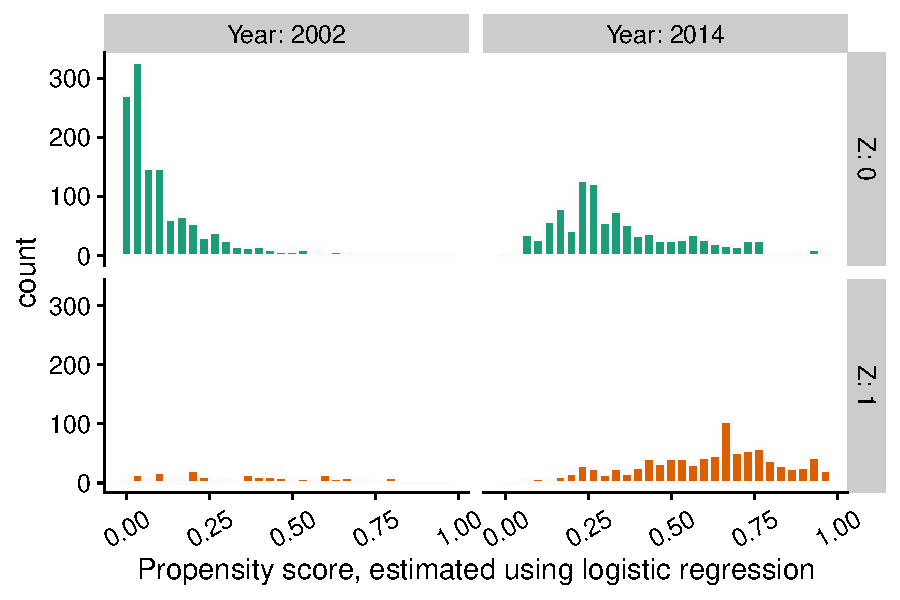
\includegraphics[width=0.6\textwidth]{figures/prop-count-logistic.pdf}
    \caption{\label{fig:propensity-logistic} Propensity scores for
      treated and untreated units for both years in the study.  These
      are estimated from logistic regression of $Z$ (\texttt{Tx}) on
      all the other covariates in Table~\ref{tab:data-description}
      (aside from \texttt{Outcome}).  % We show two histograms with
      % distinct $y$-axes, one using counts (\emph{left}), and one using
      % density (\emph{right}) to account for imbalance between the
      % quantity of observations with $Z_i=0$ and $Z_i=1$ in the
      % dataset.
      % \sw{Add a rug of discarded $Z=1$ units when using a
      % caliper, and indicators of subclassification\ldots}
    }
  \end{figure}
\item
  % -------------------------------------------------------------------------
  % B
  % -------------------------------------------------------------------------
  \begin{quoting}
    Conduct a 1-1 nearest neighbor propensity score matching procedure
    without replacement
  \end{quoting}
  % -------------------------------------------------------------------------
  As in Exercise 1, and throughout the rest of this problem, we use the
  linear model in Eq.~\eqref{eq:lin-mod} to estimate the treatment
  effect.  We use matching without replacement, matching each treated
  unit to a control unit.  Then these matched pairs are used to
  estimate the parameters of the linear model.  Thus we estimate the
  average treatment effect on the treated (ATT), 
  \begin{itemize}
  \item 2002: -1.1098 (SE = 0.0832, $p < 0.0001$) using 226 matched
    pairs
  \item 2014: -0.7262 (SE = 0.0443, $p < 0.0001$) using 921 matched
    pairs
  \end{itemize}
  As before in Exercise 1, there is a significant negative effect
  detected for both years, and the effect is larger in magnitude for
  year 2002.  Also, the estimated effect for year 2002 is larger than
  it was for the crude analysis.  Tables~\ref{tab:lm-2b-02} and
  \ref{tab:lm-2b-14} provide the full results of the linear model.

  Tables~\ref{tab-bal2b-02} and \ref{tab-bal2b-14} below provide the
  balance assessment.  For year 2002, there is a remarkable gain in
  covariate balance from matching.  Whereas many covariates appeared
  imbalanced in the crude analysis of Exercise 1 (represented by small
  p-values for the null hypothesis of equivalent covariate means
  between treated and control units), now only the covariate totOpTime
  has a significant p-value at the 95\% level.  However, for year 2014
  there is still quite substantial covariate imbalance; only the
  p-value for coal\_no\_scrubber is insignificant.

  

  \begin{table}[ht]
    \centering
    \begin{tabular}{lllrr}
      \toprule
      variable & variable.type & significance.test & test.statistic & p.value \\ 
      \midrule
      totOpTime & continuous & t-test, difference in means & -2.005 & 0.0456 \\ 
      HeatInput & continuous & t-test, difference in means & -1.307 & 0.1919 \\ 
      pctCapacity & continuous & t-test, difference in means & -1.679 & 0.0939 \\ 
      Phase2 & binary & z-test, difference in proportion & 0.053 & 0.8174 \\ 
      avgNOxControls & continuous & t-test, difference in means & -0.581 & 0.5617 \\ 
      coal\_no\_scrubber & binary & z-test, difference in proportion & 0.616 & 0.4326 \\ 
      coal\_with\_scrubber & binary & z-test, difference in proportion & 0.554 & 0.4566 \\ 
      EPA.Region & categorical & chi-sq test of independence & 5.318 & 0.8057 \\ 
      \bottomrule
    \end{tabular}
    \caption{Covariate balance check for one-to-one propensity score matching (Exercise 2(b)), year 2002} 
    \label{tab-bal2b-02}
  \end{table}

  \begin{table}[ht]
    \centering
    \begin{tabular}{lllrr}
      \toprule
      variable & variable.type & significance.test & test.statistic & p.value \\ 
      \midrule
      totOpTime & continuous & t-test, difference in means & 6.691 & $<$ 0.0001 \\ 
      HeatInput & continuous & t-test, difference in means & 5.768 & $<$ 0.0001 \\ 
      pctCapacity & continuous & t-test, difference in means & 8.138 & $<$ 0.0001 \\ 
      Phase2 & binary & z-test, difference in proportion & 32.167 & $<$ 0.0001 \\ 
      avgNOxControls & continuous & t-test, difference in means & -4.288 & $<$ 0.0001 \\ 
      coal\_no\_scrubber & binary & z-test, difference in proportion & 34.534 & $<$ 0.0001 \\ 
      coal\_with\_scrubber & binary & z-test, difference in proportion & 1.932 & 0.1645 \\ 
      EPA.Region & categorical & chi-sq test of independence & 150.241 & $<$ 0.0001 \\ 
      \bottomrule
    \end{tabular}
    \caption{Covariate balance check for one-to-one propensity score matching (Exercise 2(b)), year 2014} 
    \label{tab-bal2b-14}
  \end{table}

\item
  % -------------------------------------------------------------------------
  % C
  % -------------------------------------------------------------------------
  \begin{quoting}
    Conduct a 1-1 nearest neighbor propensity score matching procedure
    without replacement and a caliper set to 0.1 standard deviations
    of the estimated propensity score distribution.
  \end{quoting}
  % -------------------------------------------------------------------------
  After using a caliper to obtain matched pairs, the ATT estimates are
  now
  \begin{itemize}
  \item 2002: -0.9699 (SE = $0.0944$, $p < 0.0001$) using 166 matched
    pairs (60 unmatched treatment units)
  \item 2014: -0.7576 (SE $= 0.0554$, $p < 0.0001$) using 496 matched
    pairs (425 unmatched treatment units)
  \end{itemize}
  As before, there is a significant negative effect detected for both
  years, and the effect is larger in magnitude for year 2002.
  Tables~\ref{tab:lm-2c-02} and \ref{tab:lm-2c-14} provide the full
  results of the linear model.

  Tables~\ref{tab-bal2c-02} and \ref{tab-bal2c-14} show the covariate
  balance checks.  In this case, every covariate appears to be
  balanced for each year because every p-value is insignificant,
  demonstrating the advantages of using a caliper.  However, this
  comes at a price of discarding a sizable portion unmatched treatment
  units in the estimation of the treatment effect, leading to notably
  larger standard errors.

  


  \begin{table}[ht]
    \centering
    \begin{tabular}{lllrr}
      \toprule
      variable & variable.type & significance.test & test.statistic & p.value \\ 
      \midrule
      totOpTime & continuous & t-test, difference in means & -0.119 & 0.9054 \\ 
      HeatInput & continuous & t-test, difference in means & 0.253 & 0.8007 \\ 
      pctCapacity & continuous & t-test, difference in means & -0.039 & 0.9692 \\ 
      Phase2 & binary & z-test, difference in proportion & 0.016 & 0.8979 \\ 
      avgNOxControls & continuous & t-test, difference in means & 0.616 & 0.5382 \\ 
      coal\_no\_scrubber & binary & z-test, difference in proportion & 0.000 & 1.0000 \\ 
      coal\_with\_scrubber & binary & z-test, difference in proportion & 0.161 & 0.6880 \\ 
      EPA.Region & categorical & chi-sq test of independence & 5.633 & 0.7760 \\ 
      \bottomrule
    \end{tabular}
    \caption{Covariate balance check for one-to-one propensity score
      matching with a caliper (Exercise 2(c)), year 2002}
    \label{tab-bal2c-02}
  \end{table}

  \begin{table}[ht]
    \centering
    \begin{tabular}{lllrr}
      \toprule
      variable & variable.type & significance.test & test.statistic & p.value \\ 
      \midrule
      totOpTime & continuous & t-test, difference in means & -0.881 & 0.3784 \\ 
      HeatInput & continuous & t-test, difference in means & -0.527 & 0.5986 \\ 
      pctCapacity & continuous & t-test, difference in means & -1.071 & 0.2846 \\ 
      Phase2 & binary & z-test, difference in proportion & 0.243 & 0.6219 \\ 
      avgNOxControls & continuous & t-test, difference in means & -0.125 & 0.9002 \\ 
      coal\_no\_scrubber & binary & z-test, difference in proportion & 0.294 & 0.5878 \\ 
      coal\_with\_scrubber & binary & z-test, difference in proportion & 0.000 & 1.0000 \\ 
      EPA.Region & categorical & chi-sq test of independence & 8.839 & 0.4523 \\ 
      \bottomrule
    \end{tabular}
    \caption{Covariate balance check for one-to-one propensity score
      matching with a caliper (Exercise 2(c)), year 2014}
    \label{tab-bal2c-14}
  \end{table}

  % \begin{table}[ht]
  %   \centering
  %   \begin{tabular}{lllrr}
  %     \toprule
  %     variable & variable.type & significance.test & test.statistic & p.value \\ 
  %     \midrule
  %     totOpTime & continuous & t-test, difference in means & 6.691 & $<$ 0.0001 \\ 
  %     HeatInput & continuous & t-test, difference in means & 5.768 & $<$ 0.0001 \\ 
  %     pctCapacity & continuous & t-test, difference in means & 8.138 & $<$ 0.0001 \\ 
  %     Phase2 & binary & z-test, difference in proportion & 32.167 & $<$ 0.0001 \\ 
  %     avgNOxControls & continuous & t-test, difference in means & -4.288 & $<$ 0.0001 \\ 
  %     coal\_no\_scrubber & binary & z-test, difference in proportion & 34.534 & $<$ 0.0001 \\ 
  %     coal\_with\_scrubber & binary & z-test, difference in proportion & 1.932 & 0.1645 \\ 
  %     EPA.Region & categorical & chi-sq test of independence & 150.241 & $<$ 0.0001 \\ 
  %     \bottomrule
  %   \end{tabular}
  %   \caption{Covariate balance check for one-to-one propensity score
  %   matching with a caliper (Exercise 2(c)), year 2014}
  %   \label{tab-bal2c-14}
  % \end{table}


\item
  % -------------------------------------------------------------------------
  % D
  % -------------------------------------------------------------------------
  \begin{quoting}
    Conduct an analysis that subclassifies units based on the
    estimated propensity score
  \end{quoting}
  % -------------------------------------------------------------------------
  Here we use subclassification based on the propensity score
  estimated from logistic regression, creating 4 subgroups.  We again
  use a linear model for estimating the treatment effect, and use a
  weighted estimate using the sizes of the subgroups as weights (and
  also calculate a weighted estimate of the standard error in the same
  manner).
  \begin{itemize}
  \item 2002: -0.6381 (SE = 0.1285)
  \item 2014: -0.7314 (SE = 0.0890)
  \end{itemize}
  As before, there is a significant negative effect detected for both
  years.  Now, however, the effect is slightly larger in magnitude for
  year 2014 than for year 2002.

  Tables~\ref{tab-bal2d-02} and \ref{tab-bal2d-14} contain covariate
  balance diagnostics, with each column containing the p-values for
  each subgroup.  For the 2002 data, there are several instances of
  imbalance suggested by small p-values for the tests of null
  hypothesis of balance between control and treatment groups.
  This problem is even worse with the 2014 data.  Using a greater
  number of subgroups might mitigate this problem.

  \begin{table}[ht]
    \centering
    \begin{tabular}{lrrrr}
      \toprule
      variable             & subgroup1 & subgroup2 & subgroup3  & subgroup4 \\ 
      \midrule
      totOpTime            & 0.5071    & 0.1241    & $<$ 0.0001 & 0.3076    \\ 
      HeatInput            & 0.4012    & 0.6007    & 0.0029     & 0.1101    \\ 
      pctCapacity          & 0.9979    & 0.3034    & 0.0012     & 0.3677    \\ 
      Phase2               & 1.0000    & 1.0000    & 0.5589     & 0.2496    \\ 
      avgNOxControls       & 0.0337    & 0.0361    & 0.2993     & 0.9215    \\ 
      coal\_no\_scrubber   & 0.0194    & 1.0000    & 0.8819     & 1.0000    \\ 
      coal\_with\_scrubber & 0.5845    & 0.8112    & 0.1682     & 1.0000        \\ 
      EPA.Region           & 0.0002    & 0.0104    & 0.2480     & 0.0530    \\ 
      \bottomrule
    \end{tabular}
    \caption{Covariate balance check for subclassification using propensity score (4 subclasses), year 2002} 
    \label{tab-bal2d-02}
  \end{table}

  \begin{table}[ht]
    \centering
    \begin{tabular}{lrrrr}
      \toprule
      variable & subgroup1 & subgroup2 & subgroup3 & subgroup4 \\ 
      \midrule
      totOpTime & $<$ 0.0001 & 0.0013 & 0.0017 & 0.0329 \\ 
      HeatInput & $<$ 0.0001 & 0.2439 & 0.7289 & 0.0812 \\ 
      pctCapacity & $<$ 0.0001 & 0.0004 & 0.0059 & 0.1802 \\ 
      Phase2 & 0.4905 & 0.2273 & 0.8723 & 1.0000 \\ 
      avgNOxControls & 0.9718 & 0.6884 & 0.0005 & $<$ 0.0001 \\ 
      coal\_no\_scrubber & 0.7270 & 0.1304 & 0.5050 & 0.4342 \\ 
      coal\_with\_scrubber & $<$ 0.0001 & 0.6324 & 0.9029 & $<$ 0.0001 \\ 
      EPA.Region & 0.0006 & $<$ 0.0001 & 0.0036 & 0.0983 \\ 
      \bottomrule
    \end{tabular}
    \caption{Covariate balance check for subclassification using propensity score (4 subclasses), year 2014} 
    \label{tab-bal2d-14}
  \end{table}

\item
  % -------------------------------------------------------------------------
  % E
  % -------------------------------------------------------------------------
  \begin{quoting}
    Conduct an IPW analysis using weights
    $\frac{W_i}{\hat e(X_i)} + \frac{1 - W_i}{1 - \hat e(X_i)}$ and be
    sure to include a visual summary (e.g., histogram) of the
    estimated weights.
  \end{quoting}
  % -------------------------------------------------------------------------

  We calculate the weights as described, using the propensity score
  estimated from logistic regression as $\hat e(X_i)$.  We fit a
  weighted least squares estimate of the linear model in
  Eq.~\eqref{eq:lin-mod} using the \texttt{lm} command in R.
  \begin{itemize}
  \item 2002: -0.5951 (SE = 0.0404)
  \item 2014: -0.6447 (SE = 0.0404)
  \end{itemize}
  There is a significant negative effect detected for both years, and
  the effect is slightly larger in magnitude for year 2014 than for
  year 2002.  Full results from the regression are presented presented
  in Tables~\ref{tab:lm-2e-02} and \ref{tab:lm-2e-14} at the end of
  the document.
  
  Figure~\ref{fig:weights} shows a visualization of the weights
  arranged by their magnitude and colored by treatment assignment.  We
  notice that there are several observations with weights which are
  strikingly large, and therefore these weights may dominate the
  eventual estimated causal effects. 

  

  \begin{figure}[ht]
    \centering
    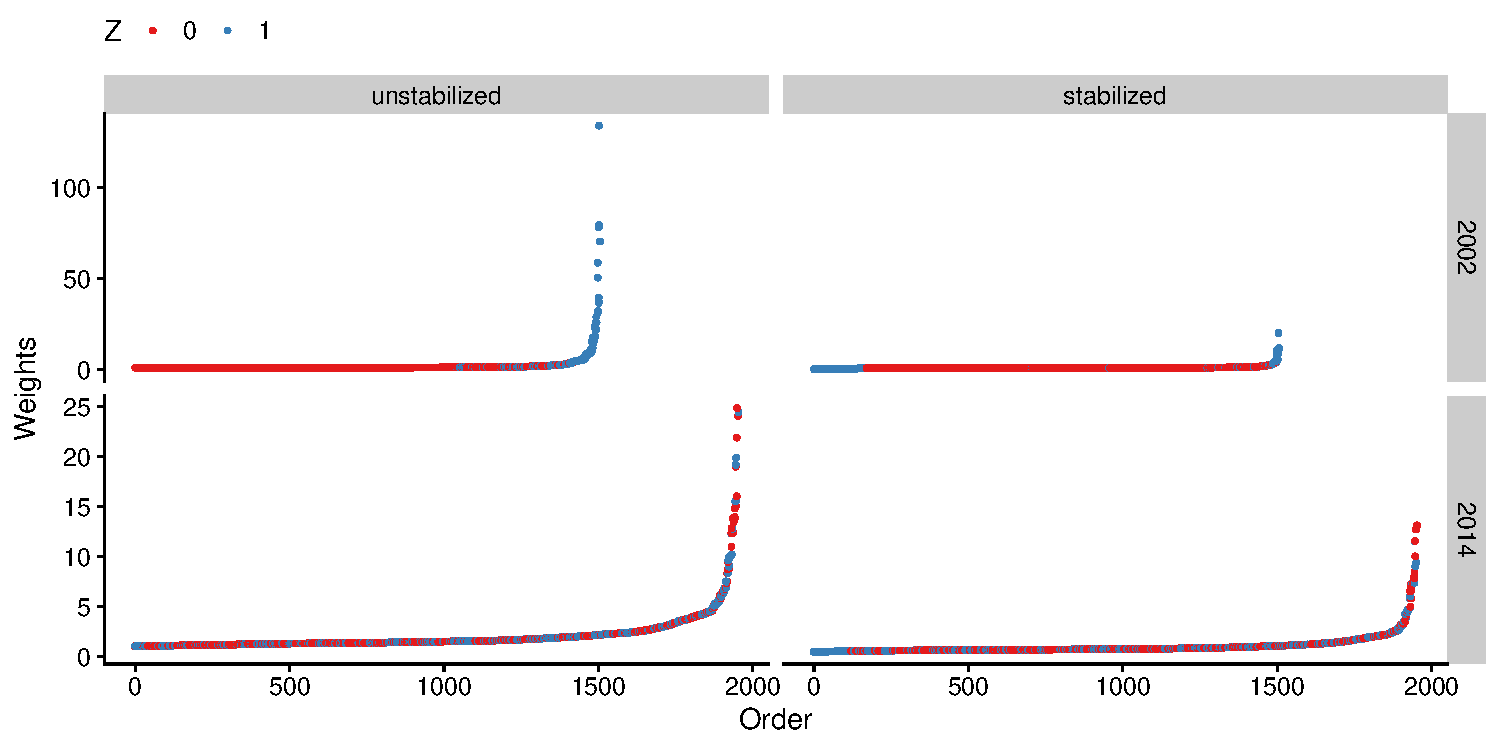
\includegraphics[width=\textwidth]{figures/weights-all.pdf}
    \caption{\label{fig:weights} Unstabilized and stabilized inverse
      probability weights for Exercises (2e) and (2f). }
  \end{figure}


\item
  % -------------------------------------------------------------------------
  % F
  % -------------------------------------------------------------------------
  \begin{quoting}
    Conduct an IPW analysis using stabilized weights and be sure to
    include a visual summary (e.g., histogram) of the estimated
    weights.
  \end{quoting}
  % -------------------------------------------------------------------------
  Now the weights become
  $\frac{W_i \cdot \hat \Pr(W_i = 1)}{\hat e(X_i)} + \frac{(1 - W_i)
    \cdot \hat \Pr(W_i = 0)}{1 - \hat e(X_i)}$ where $\Pr(W_i = 1)$ is
  the marginal probability of assignment to treatment.  That is,
  $\hat \Pr(W_i = 1)$ is the sample proportion of units which receive
  treatment.  These stabilized weights are compared to the stabilized
  weights in Figure \ref{fig:prop-comp}.  We can see how the variance
  of the weights is reduced in this manner.  
  \begin{itemize}
  \item 2002: -0.5349 (SE = 0.0572)
  \item 2014: -0.6432 (SE = 0.0407)
  \end{itemize}
  There is a significant negative effect detected for both years, and
  the effect is slightly larger in magnitude for year 2014 than for
  year 2002.  However, even though the weights themselves have lower
  variance, the standard errors for the estimated causal effects are
  slightly larger than they were for the analysis using unstabilized
  weights.  Full regression results are given in
  Tables~\ref{tab:lm-2f-02} and \ref{tab:lm-2f-14} at the end of the
  document.

\end{enumerate}

%%% Local Variables:
%%% mode: latex
%%% TeX-master: "../main"
%%% End:


% \pagebreak


\section{Exercise 3}

\begin{quoting}
  Describe in $\sim$5 sentences why the answers you obtained with the
  different propensity score methods in Exercise (2) were different
  from one another.
\end{quoting}

Every analysis in Exercise 2 used a linear model to estimate the
causal effect of SnCR installation on log-emissions of NO$_x$.
However, the estimates differed considerably.  This is all due to how
observations were either selected or weighted.  That is, matching,
both with and without a caliper, removed many observations from
consideration when estimating the parameters of the linear model in
Eq.~\eqref{eq:lin-mod} because there were not any units with
adequately similar propensity scores to these units.  Alternatively,
the IPW analyses included every observation in the analysis, but
weighted each one differently.  Finally, the subclassification
analysis also included every unit, but weighted each one according to
the size of the subclassiciation (based on the estimated propensity
score) to which it belonged.

%%% Local Variables:
%%% mode: latex
%%% TeX-master: "../main"
%%% End:


% \pagebreak


\section{Exercise 4}

\begin{quoting}
  Repeat Exercise (1e), but use a more advanced prediction model (your
  choice) to estimate the propensity score. Describe ($\sim$3
  sentences) any differences.
\end{quoting}

%%% Local Variables:
%%% mode: latex
%%% TeX-master: "../main"
%%% End:



\section{Additional tables and figures}

% -------------------------------------------------------------------------
% Problem 1

\begin{table}[ht]
\centering
\begin{tabular}{lrrrr}
  \toprule
                       & Estimate & Std. Error & t value & Pr($>$$|$t$|$) \\ 
  \midrule
(Intercept)            & 3.1269   & 0.1261     & 24.80   & 0.0000         \\ \midrule
  Tx                   & -0.9525  & 0.0669     & -14.23  & 0.0000         \\ \midrule
  totOpTime            & 0.0003   & 0.0000     & 20.27   & 0.0000         \\ 
  HeatInput            & 0.0000   & 0.0000     & 26.03   & 0.0000         \\ 
  pctCapacity          & -0.5005  & 0.1727     & -2.90   & 0.0038         \\ 
  Phase2               & -0.0635  & 0.0581     & -1.09   & 0.2747         \\ 
  avgNOxControls       & -0.1118  & 0.0427     & -2.62   & 0.0089         \\ 
  coal\_no\_scrubber   & 1.7313   & 0.0673     & 25.74   & 0.0000         \\ 
  coal\_with\_scrubber & 1.6007   & 0.0937     & 17.09   & 0.0000         \\ 
  EPA.Region2          & -0.1837  & 0.1136     & -1.62   & 0.1060         \\ 
  EPA.Region3          & 0.0960   & 0.1131     & 0.85    & 0.3962         \\ 
  EPA.Region4          & 0.1514   & 0.1060     & 1.43    & 0.1534         \\ 
  EPA.Region5          & -0.0944  & 0.1113     & -0.85   & 0.3964         \\ 
  EPA.Region6          & 0.1331   & 0.1124     & 1.18    & 0.2362         \\ 
  EPA.Region7          & -0.1584  & 0.1377     & -1.15   & 0.2501         \\ 
  EPA.Region8          & -0.0929  & 0.1377     & -0.67   & 0.5001         \\ 
  EPA.Region9          & -0.3204  & 0.1256     & -2.55   & 0.0108         \\ 
  EPA.Region10         & -0.1175  & 0.3222     & -0.36   & 0.7153         \\ 
   \bottomrule
\end{tabular}
\caption{``Crude'' linear regression model for estimating of treatment
  effect using 2002 data}
\label{tab:crude-lm-02}
\end{table}


\begin{table}[ht]
\centering
\begin{tabular}{lrrrr}
  \toprule
                       & Estimate & Std. Error & t value & Pr($>$$|$t$|$) \\ 
  \midrule
(Intercept)            & 2.3451   & 0.1263     & 18.57   & 0.0000         \\  \midrule
  Tx                   & -0.7069  & 0.0450     & -15.72  & 0.0000         \\  \midrule
  totOpTime            & 0.0004   & 0.0000     & 18.85   & 0.0000         \\ 
  HeatInput            & 0.0000   & 0.0000     & 17.57   & 0.0000         \\ 
  pctCapacity          & -0.6875  & 0.2424     & -2.84   & 0.0046         \\ 
  Phase2               & -0.1244  & 0.0556     & -2.24   & 0.0255         \\ 
  avgNOxControls       & -0.2243  & 0.0386     & -5.81   & 0.0000         \\ 
  coal\_no\_scrubber   & 2.0186   & 0.0833     & 24.22   & 0.0000         \\ 
  coal\_with\_scrubber & 1.9837   & 0.0809     & 24.51   & 0.0000         \\ 
  EPA.Region2          & 0.0422   & 0.1298     & 0.32    & 0.7453         \\ 
  EPA.Region3          & 0.0476   & 0.1272     & 0.37    & 0.7082         \\ 
  EPA.Region4          & 0.0133   & 0.1191     & 0.11    & 0.9111         \\ 
  EPA.Region5          & -0.0205  & 0.1234     & -0.17   & 0.8682         \\ 
  EPA.Region6          & 0.2671   & 0.1220     & 2.19    & 0.0287         \\ 
  EPA.Region7          & 0.0379   & 0.1465     & 0.26    & 0.7961         \\ 
  EPA.Region8          & -0.1861  & 0.1491     & -1.25   & 0.2120         \\ 
  EPA.Region9          & -0.7299  & 0.1240     & -5.89   & 0.0000         \\ 
  EPA.Region10         & -0.1352  & 0.2280     & -0.59   & 0.5531         \\ 
   \bottomrule
\end{tabular}
\caption{``Crude'' linear regression model for estimating of treatment
  effect using 2014 data}
\label{tab:crude-lm-14}
\end{table}

% -------------------------------------------------------------------------
% Problem 2(b)



\begin{table}[ht]
\centering
\begin{tabular}{lrrrr}
  \toprule
 & Estimate & Std. Error & t value & Pr($>$$|$t$|$) \\ 
  \midrule
(Intercept) & 3.3332 & 0.1859 & 17.93 & 0.0000 \\ 
  Z02B & -1.1098 & 0.0832 & -13.34 & 0.0000 \\ 
  totOpTime & 0.0003 & 0.0000 & 9.67 & 0.0000 \\ 
  HeatInput & 0.0000 & 0.0000 & 10.87 & 0.0000 \\ 
  pctCapacity & -0.9851 & 0.3778 & -2.61 & 0.0094 \\ 
  Phase2 & -0.0967 & 0.1190 & -0.81 & 0.4171 \\ 
  avgNOxControls & -0.0534 & 0.0838 & -0.64 & 0.5241 \\ 
  coal\_no\_scrubber & 1.8828 & 0.1546 & 12.18 & 0.0000 \\ 
  coal\_with\_scrubber & 1.8678 & 0.1952 & 9.57 & 0.0000 \\ 
  EPA.Region2 & -0.0801 & 0.1383 & -0.58 & 0.5628 \\ 
  EPA.Region3 & 0.2501 & 0.1679 & 1.49 & 0.1371 \\ 
  EPA.Region4 & 0.2099 & 0.1532 & 1.37 & 0.1712 \\ 
  EPA.Region5 & 0.1218 & 0.2445 & 0.50 & 0.6186 \\ 
  EPA.Region6 & 0.0095 & 0.1634 & 0.06 & 0.9538 \\ 
  EPA.Region7 & -0.0014 & 0.4712 & -0.00 & 0.9977 \\ 
  EPA.Region8 & -0.1420 & 0.6301 & -0.23 & 0.8217 \\ 
  EPA.Region9 & -0.3774 & 0.1470 & -2.57 & 0.0106 \\ 
  EPA.Region10 & -0.1678 & 0.3545 & -0.47 & 0.6362 \\ 
   \bottomrule
\end{tabular}
\caption{Linear regression model for estimating of treatment effect using 2002 data, after using one-to-one matching (Problem 2(b))} 
\label{tab:lm-2b-02}
\end{table}

\begin{table}[ht]
\centering
\begin{tabular}{lrrrr}
  \toprule
 & Estimate & Std. Error & t value & Pr($>$$|$t$|$) \\ 
  \midrule
(Intercept) & 2.4951 & 0.1272 & 19.61 & 0.0000 \\ 
  Z14B & -0.7262 & 0.0443 & -16.40 & 0.0000 \\ 
  totOpTime & 0.0004 & 0.0000 & 18.86 & 0.0000 \\ 
  HeatInput & 0.0000 & 0.0000 & 17.38 & 0.0000 \\ 
  pctCapacity & -0.8106 & 0.2432 & -3.33 & 0.0009 \\ 
  Phase2 & -0.2393 & 0.0608 & -3.93 & 0.0001 \\ 
  avgNOxControls & -0.2479 & 0.0389 & -6.37 & 0.0000 \\ 
  coal\_no\_scrubber & 2.0182 & 0.0872 & 23.14 & 0.0000 \\ 
  coal\_with\_scrubber & 2.0067 & 0.0817 & 24.57 & 0.0000 \\ 
  EPA.Region2 & 0.0125 & 0.1277 & 0.10 & 0.9223 \\ 
  EPA.Region3 & 0.0909 & 0.1257 & 0.72 & 0.4698 \\ 
  EPA.Region4 & 0.0552 & 0.1174 & 0.47 & 0.6384 \\ 
  EPA.Region5 & -0.0282 & 0.1221 & -0.23 & 0.8175 \\ 
  EPA.Region6 & 0.2705 & 0.1213 & 2.23 & 0.0259 \\ 
  EPA.Region7 & 0.1066 & 0.1546 & 0.69 & 0.4908 \\ 
  EPA.Region8 & -0.1946 & 0.1493 & -1.30 & 0.1926 \\ 
  EPA.Region9 & -0.7155 & 0.1219 & -5.87 & 0.0000 \\ 
  EPA.Region10 & -0.1188 & 0.2241 & -0.53 & 0.5959 \\ 
   \bottomrule
\end{tabular}
\caption{Linear regression model for estimating of treatment effect using 2014 data, after using one-to-one matching (Problem 2(b))} 
\label{tab:lm-2b-14}
\end{table}

% -------------------------------------------------------------------------
% Problem 2c

\begin{table}[ht]
\centering
\begin{tabular}{lrrrr}
  \toprule
 & Estimate & Std. Error & t value & Pr($>$$|$t$|$) \\ 
  \midrule
(Intercept) & 3.1323 & 0.2012 & 15.57 & 0.0000 \\ 
  Z02C & -0.9699 & 0.0944 & -10.28 & 0.0000 \\ 
  totOpTime & 0.0003 & 0.0000 & 7.99 & 0.0000 \\ 
  HeatInput & 0.0000 & 0.0000 & 10.10 & 0.0000 \\ 
  pctCapacity & -0.5376 & 0.4134 & -1.30 & 0.1943 \\ 
  Phase2 & -0.0358 & 0.1311 & -0.27 & 0.7849 \\ 
  avgNOxControls & -0.0580 & 0.0974 & -0.60 & 0.5520 \\ 
  coal\_no\_scrubber & 2.1735 & 0.1637 & 13.28 & 0.0000 \\ 
  coal\_with\_scrubber & 1.8272 & 0.2172 & 8.41 & 0.0000 \\ 
  EPA.Region2 & 0.0156 & 0.1621 & 0.10 & 0.9236 \\ 
  EPA.Region3 & 0.0241 & 0.1795 & 0.13 & 0.8934 \\ 
  EPA.Region4 & 0.0796 & 0.1767 & 0.45 & 0.6525 \\ 
  EPA.Region5 & 0.2477 & 0.2577 & 0.96 & 0.3371 \\ 
  EPA.Region6 & 0.0560 & 0.1846 & 0.30 & 0.7620 \\ 
  EPA.Region7 & -0.0550 & 0.3824 & -0.14 & 0.8857 \\ 
  EPA.Region8 & -0.7518 & 0.6312 & -1.19 & 0.2346 \\ 
  EPA.Region9 & -0.2674 & 0.1889 & -1.42 & 0.1579 \\ 
  EPA.Region10 & -1.0731 & 0.9009 & -1.19 & 0.2345 \\ 
   \bottomrule
\end{tabular}
\caption{Linear regression model for estimating of treatment effect
  using 2002 data, after using one-to-one matching with a caliber
  (Problem 2(c))}
\label{tab:lm-2c-02}
\end{table}

\begin{table}[ht]
\centering
\begin{tabular}{lrrrr}
  \toprule
 & Estimate & Std. Error & t value & Pr($>$$|$t$|$) \\ 
  \midrule
(Intercept) & 2.2247 & 0.2020 & 11.01 & 0.0000 \\ 
  Z14C & -0.7576 & 0.0554 & -13.67 & 0.0000 \\ 
  totOpTime & 0.0004 & 0.0000 & 13.79 & 0.0000 \\ 
  HeatInput & 0.0000 & 0.0000 & 13.71 & 0.0000 \\ 
  pctCapacity & -0.8967 & 0.3137 & -2.86 & 0.0043 \\ 
  Phase2 & -0.1476 & 0.0838 & -1.76 & 0.0787 \\ 
  avgNOxControls & -0.2089 & 0.0531 & -3.94 & 0.0001 \\ 
  coal\_no\_scrubber & 2.1244 & 0.1200 & 17.71 & 0.0000 \\ 
  coal\_with\_scrubber & 2.0743 & 0.1066 & 19.46 & 0.0000 \\ 
  EPA.Region2 & 0.3108 & 0.2032 & 1.53 & 0.1264 \\ 
  EPA.Region3 & 0.4681 & 0.2045 & 2.29 & 0.0223 \\ 
  EPA.Region4 & 0.3958 & 0.1947 & 2.03 & 0.0423 \\ 
  EPA.Region5 & 0.3375 & 0.1982 & 1.70 & 0.0890 \\ 
  EPA.Region6 & 0.4620 & 0.1950 & 2.37 & 0.0180 \\ 
  EPA.Region7 & 0.3952 & 0.2372 & 1.67 & 0.0959 \\ 
  EPA.Region8 & -0.0833 & 0.2218 & -0.38 & 0.7072 \\ 
  EPA.Region9 & -0.4709 & 0.2047 & -2.30 & 0.0216 \\ 
  EPA.Region10 & -0.7215 & 0.3992 & -1.81 & 0.0710 \\ 
   \bottomrule
\end{tabular}
\caption{Linear regression model for estimating of treatment effect using 2014 data, after using one-to-one matching with a caliber (Problem 2(c))} 
\label{tab:lm-2c-14}
\end{table}

% -------------------------------------------------------------------------
% E

\begin{table}[ht]
\centering
\begin{tabular}{lrrrr}
  \toprule
 & Estimate & Std. Error & t value & Pr($>$$|$t$|$) \\ 
  \midrule
(Intercept) & 3.1828 & 0.1129 & 28.20 & 0.0000 \\ 
  Z02 & -0.5951 & 0.0404 & -14.73 & 0.0000 \\ 
  totOpTime & 0.0003 & 0.0000 & 18.70 & 0.0000 \\ 
  HeatInput & 0.0000 & 0.0000 & 30.09 & 0.0000 \\ 
  pctCapacity & -0.7127 & 0.1780 & -4.00 & 0.0001 \\ 
  Phase2 & -0.1846 & 0.0525 & -3.52 & 0.0005 \\ 
  avgNOxControls & -0.0141 & 0.0383 & -0.37 & 0.7122 \\ 
  coal\_no\_scrubber & 2.0877 & 0.0673 & 31.02 & 0.0000 \\ 
  coal\_with\_scrubber & 1.8016 & 0.0861 & 20.92 & 0.0000 \\ 
  EPA.Region2 & -0.1740 & 0.1062 & -1.64 & 0.1016 \\ 
  EPA.Region3 & 0.2463 & 0.1024 & 2.40 & 0.0163 \\ 
  EPA.Region4 & 0.1218 & 0.0965 & 1.26 & 0.2073 \\ 
  EPA.Region5 & -0.0723 & 0.1008 & -0.72 & 0.4737 \\ 
  EPA.Region6 & 0.0904 & 0.1037 & 0.87 & 0.3833 \\ 
  EPA.Region7 & -0.0247 & 0.1303 & -0.19 & 0.8498 \\ 
  EPA.Region8 & -0.2829 & 0.1374 & -2.06 & 0.0396 \\ 
  EPA.Region9 & -0.3766 & 0.1209 & -3.12 & 0.0019 \\ 
  EPA.Region10 & -0.2326 & 0.3523 & -0.66 & 0.5091 \\ 
   \bottomrule
\end{tabular}
\caption{Linear regression model with inverse probability weights for estimating of treatment effect using 2002 data (Problem 2(e))} 
\label{tab:lm-2e-02}
\end{table}

\begin{table}[ht]
\centering
\begin{tabular}{lrrrr}
  \toprule
 & Estimate & Std. Error & t value & Pr($>$$|$t$|$) \\ 
  \midrule
(Intercept) & 2.3423 & 0.1311 & 17.87 & 0.0000 \\ 
  Z14 & -0.6447 & 0.0404 & -15.96 & 0.0000 \\ 
  totOpTime & 0.0004 & 0.0000 & 19.95 & 0.0000 \\ 
  HeatInput & 0.0000 & 0.0000 & 16.73 & 0.0000 \\ 
  pctCapacity & -0.5570 & 0.2084 & -2.67 & 0.0076 \\ 
  Phase2 & -0.1954 & 0.0584 & -3.34 & 0.0008 \\ 
  avgNOxControls & -0.1584 & 0.0392 & -4.04 & 0.0001 \\ 
  coal\_no\_scrubber & 2.4075 & 0.0803 & 29.97 & 0.0000 \\ 
  coal\_with\_scrubber & 2.3278 & 0.0768 & 30.32 & 0.0000 \\ 
  EPA.Region2 & 0.0331 & 0.1329 & 0.25 & 0.8032 \\ 
  EPA.Region3 & 0.1329 & 0.1289 & 1.03 & 0.3029 \\ 
  EPA.Region4 & 0.0253 & 0.1217 & 0.21 & 0.8355 \\ 
  EPA.Region5 & -0.0472 & 0.1255 & -0.38 & 0.7069 \\ 
  EPA.Region6 & 0.1828 & 0.1232 & 1.48 & 0.1380 \\ 
  EPA.Region7 & 0.3232 & 0.1465 & 2.21 & 0.0275 \\ 
  EPA.Region8 & -0.4678 & 0.1449 & -3.23 & 0.0013 \\ 
  EPA.Region9 & -0.7337 & 0.1245 & -5.89 & 0.0000 \\ 
  EPA.Region10 & -0.1528 & 0.2527 & -0.60 & 0.5455 \\ 
   \bottomrule
\end{tabular}
\caption{Linear regression model with inverse probability weights for estimating of treatment effect using 2014 data (Problem 2(e))} 
\label{tab:lm-2e-14}
\end{table}

% -------------------------------------------------------------------------
% F

\begin{table}[ht]
\centering
\begin{tabular}{lrrrr}
  \toprule
 & Estimate & Std. Error & t value & Pr($>$$|$t$|$) \\ 
  \midrule
(Intercept) & 3.2503 & 0.1151 & 28.23 & 0.0000 \\ 
  Z02 & -0.5349 & 0.0572 & -9.36 & 0.0000 \\ 
  totOpTime & 0.0003 & 0.0000 & 20.27 & 0.0000 \\ 
  HeatInput & 0.0000 & 0.0000 & 27.49 & 0.0000 \\ 
  pctCapacity & -0.5994 & 0.1718 & -3.49 & 0.0005 \\ 
  Phase2 & -0.0699 & 0.0559 & -1.25 & 0.2112 \\ 
  avgNOxControls & -0.0864 & 0.0410 & -2.11 & 0.0351 \\ 
  coal\_no\_scrubber & 1.7745 & 0.0669 & 26.53 & 0.0000 \\ 
  coal\_with\_scrubber & 1.5858 & 0.0904 & 17.53 & 0.0000 \\ 
  EPA.Region2 & -0.2973 & 0.1107 & -2.69 & 0.0073 \\ 
  EPA.Region3 & -0.0205 & 0.1078 & -0.19 & 0.8493 \\ 
  EPA.Region4 & 0.0122 & 0.1013 & 0.12 & 0.9041 \\ 
  EPA.Region5 & -0.1942 & 0.1056 & -1.84 & 0.0661 \\ 
  EPA.Region6 & -0.0441 & 0.1085 & -0.41 & 0.6841 \\ 
  EPA.Region7 & -0.2497 & 0.1336 & -1.87 & 0.0618 \\ 
  EPA.Region8 & -0.2720 & 0.1353 & -2.01 & 0.0445 \\ 
  EPA.Region9 & -0.2359 & 0.1272 & -1.85 & 0.0638 \\ 
  EPA.Region10 & -0.3239 & 0.3999 & -0.81 & 0.4181 \\ 
   \bottomrule
\end{tabular}
\caption{Linear regression model with stabilized inverse probability
  weights for estimating of treatment effect using 2002 data (Problem
  2(f))}
\label{tab:lm-2f-02}
\end{table}

\begin{table}[ht]
\centering
\begin{tabular}{lrrrr}
  \toprule
 & Estimate & Std. Error & t value & Pr($>$$|$t$|$) \\ 
  \midrule
(Intercept) & 2.3351 & 0.1314 & 17.77 & 0.0000 \\ 
  Z14 & -0.6432 & 0.0407 & -15.81 & 0.0000 \\ 
  totOpTime & 0.0004 & 0.0000 & 19.94 & 0.0000 \\ 
  HeatInput & 0.0000 & 0.0000 & 16.70 & 0.0000 \\ 
  pctCapacity & -0.5593 & 0.2079 & -2.69 & 0.0072 \\ 
  Phase2 & -0.1845 & 0.0584 & -3.16 & 0.0016 \\ 
  avgNOxControls & -0.1534 & 0.0395 & -3.89 & 0.0001 \\ 
  coal\_no\_scrubber & 2.4006 & 0.0806 & 29.77 & 0.0000 \\ 
  coal\_with\_scrubber & 2.3399 & 0.0769 & 30.41 & 0.0000 \\ 
  EPA.Region2 & 0.0487 & 0.1335 & 0.36 & 0.7153 \\ 
  EPA.Region3 & 0.1181 & 0.1294 & 0.91 & 0.3615 \\ 
  EPA.Region4 & 0.0249 & 0.1222 & 0.20 & 0.8385 \\ 
  EPA.Region5 & -0.0609 & 0.1260 & -0.48 & 0.6288 \\ 
  EPA.Region6 & 0.1914 & 0.1237 & 1.55 & 0.1221 \\ 
  EPA.Region7 & 0.2943 & 0.1473 & 2.00 & 0.0459 \\ 
  EPA.Region8 & -0.4506 & 0.1458 & -3.09 & 0.0020 \\ 
  EPA.Region9 & -0.7405 & 0.1250 & -5.92 & 0.0000 \\ 
  EPA.Region10 & -0.1873 & 0.2546 & -0.74 & 0.4619 \\ 
   \bottomrule
\end{tabular}
\caption{Linear regression model with stabilized inverse probability weights for estimating of treatment effect using 2014 data (Problem 2(f))} 
\label{tab:lm-2f-14}
\end{table}

% -------------------------------------------------------------------------
% Problem 4

\begin{table}[ht]
\centering
\begin{tabular}{lrrrr}
  \toprule
 & Estimate & Std. Error & t value & Pr($>$$|$t$|$) \\ 
  \midrule
(Intercept) & 3.1718 & 0.1165 & 27.23 & 0.0000 \\ 
  Z02 & -0.6651 & 0.0434 & -15.32 & 0.0000 \\ 
  totOpTime & 0.0003 & 0.0000 & 19.24 & 0.0000 \\ 
  HeatInput & 0.0000 & 0.0000 & 29.39 & 0.0000 \\ 
  pctCapacity & -0.7669 & 0.1769 & -4.34 & 0.0000 \\ 
  Phase2 & -0.1569 & 0.0557 & -2.82 & 0.0049 \\ 
  avgNOxControls & -0.0828 & 0.0416 & -1.99 & 0.0468 \\ 
  coal\_no\_scrubber & 1.9802 & 0.0690 & 28.69 & 0.0000 \\ 
  coal\_with\_scrubber & 1.6800 & 0.0916 & 18.34 & 0.0000 \\ 
  EPA.Region2 & -0.1415 & 0.1060 & -1.33 & 0.1822 \\ 
  EPA.Region3 & 0.2399 & 0.1045 & 2.30 & 0.0218 \\ 
  EPA.Region4 & 0.1718 & 0.0976 & 1.76 & 0.0787 \\ 
  EPA.Region5 & -0.0032 & 0.1043 & -0.03 & 0.9753 \\ 
  EPA.Region6 & 0.0617 & 0.1035 & 0.60 & 0.5514 \\ 
  EPA.Region7 & -0.1163 & 0.1349 & -0.86 & 0.3886 \\ 
  EPA.Region8 & -0.1497 & 0.1441 & -1.04 & 0.2992 \\ 
  EPA.Region9 & -0.4095 & 0.1196 & -3.42 & 0.0006 \\ 
  EPA.Region10 & -0.2244 & 0.3406 & -0.66 & 0.5102 \\ 
   \bottomrule
\end{tabular}
\caption{Linear regression model with inverse probability weights (estimated using BART) for estimating of treatment effect using 2002 data (Problem 4)} 
\label{tab:lm-2g-02}
\end{table}

\begin{table}[ht]
\centering
\begin{tabular}{lrrrr}
  \toprule
 & Estimate & Std. Error & t value & Pr($>$$|$t$|$) \\ 
  \midrule
(Intercept) & 2.2510 & 0.1222 & 18.42 & 0.0000 \\ 
  Z14 & -0.8018 & 0.0410 & -19.57 & 0.0000 \\ 
  totOpTime & 0.0004 & 0.0000 & 19.65 & 0.0000 \\ 
  HeatInput & 0.0000 & 0.0000 & 16.74 & 0.0000 \\ 
  pctCapacity & -0.9289 & 0.2388 & -3.89 & 0.0001 \\ 
  Phase2 & -0.0768 & 0.0598 & -1.29 & 0.1988 \\ 
  avgNOxControls & -0.2529 & 0.0388 & -6.52 & 0.0000 \\ 
  coal\_no\_scrubber & 2.1620 & 0.0828 & 26.12 & 0.0000 \\ 
  coal\_with\_scrubber & 2.0603 & 0.0820 & 25.13 & 0.0000 \\ 
  EPA.Region2 & 0.2323 & 0.1240 & 1.87 & 0.0612 \\ 
  EPA.Region3 & 0.2306 & 0.1192 & 1.93 & 0.0532 \\ 
  EPA.Region4 & 0.1503 & 0.1108 & 1.36 & 0.1751 \\ 
  EPA.Region5 & 0.1180 & 0.1157 & 1.02 & 0.3077 \\ 
  EPA.Region6 & 0.2884 & 0.1125 & 2.56 & 0.0104 \\ 
  EPA.Region7 & 0.3200 & 0.1419 & 2.26 & 0.0242 \\ 
  EPA.Region8 & -0.2502 & 0.1402 & -1.79 & 0.0743 \\ 
  EPA.Region9 & -0.7432 & 0.1176 & -6.32 & 0.0000 \\ 
  EPA.Region10 & 0.0426 & 0.2432 & 0.18 & 0.8610 \\ 
   \bottomrule
\end{tabular}
\caption{Linear regression model with inverse probability weights (estimated using BART) for estimating of treatment effect using 2014 data (Problem 4)} 
\label{tab:lm-2g-14}
\end{table}

%%% Local Variables:
%%% mode: latex
%%% TeX-master: "../main"
%%% End:



% -------------------------------------------------------------------------
% References

% \bibliographystyle{plainnat}
% \pagebreak




% -------------------------------------------------------------------------
% List code

% \pagebreak
% % \rscript{homework03.r}{Sample Perl R With Highlighting}
% \lstinputlisting[language=R,
% basicstyle=\footnotesize\ttfamily]{problem03.R}
 
% -------------------------------------------------------------------------
% References


\bibliographystyle{plainnat}

\begin{raggedright}
\bibliography{main}
\end{raggedright}


% -------------------------------------------------------------------------


\end{document}

%%% Local Variables:
%%% mode: latex
%%% TeX-master: t
%%% End:
